% This must be in the first 5 lines to tell arXiv to use pdfLaTeX, which is strongly recommended.
\pdfoutput=1
% In particular, the hyperref package requires pdfLaTeX in order to break URLs across lines.

\documentclass[11pt]{article}

% Remove the "review" option to generate the final version.
\usepackage[]{acl}

% Standard package includes
\usepackage{times}
\usepackage{latexsym}

% For proper rendering and hyphenation of words containing Latin characters (including in bib files)
\usepackage[T1]{fontenc}
% For Vietnamese characters
% \usepackage[T5]{fontenc}
% See https://www.latex-project.org/help/documentation/encguide.pdf for other character sets

% This assumes your files are encoded as UTF8
\usepackage[utf8]{inputenc}

% This is not strictly necessary, and may be commented out,
% but it will improve the layout of the manuscript,
% and will typically save some space.
\usepackage{microtype}
\newcommand{\bbox}{\text{bbox}}
\newcommand{\alphapck}{\alpha_\bbox}
\newcommand{\kcycle}{\text{k-CyPCK}}
\newcommand{\cycle}{\text{-CyPCK}}

\newcommand{\I}{\mathbf{I}}
\newcommand{\Ia}{\I^\text{a}}
\newcommand{\Ib}{\I^\text{b}}
\newcommand{\Iatob}{\I^\text{a $\rightarrow$ b}}
\newcommand{\F}{\mathbf{F}}
\newcommand{\Fa}{\F^\text{a}}
\newcommand{\Fb}{\F^\text{b}}
\newcommand{\f}{\mathbf{f}}
\newcommand{\fa}{\f^\text{a}}
\newcommand{\fb}{\f^\text{b}}
\newcommand{\p}{\mathbf{p}}
\newcommand{\pa}{\p^\text{a}}
\newcommand{\pb}{\p^\text{b}}
\newcommand{\A}{\boldsymbol{\Phi}_\text{align}}
\newcommand{\G}{\mathbf{G}}
\newcommand{\C}{\mathbf{C}}
\newcommand{\Ca}{\C^\text{a}}
\newcommand{\Cb}{\C^\text{b}}
\newcommand{\cc}{\mathbf{c}}
\newcommand{\cca}{\cc^\text{a}}
\newcommand{\ccb}{\cc^\text{b}}
\newcommand{\Irec}{\I_\text{Recon}}
\newcommand{\M}{\mathbf{M}}
\newcommand{\Mrec}{\M_\text{Recon}}
\newcommand{\loss}{\mathcal{L}}
\newcommand{\T}{\mathcal{T}}
\newcommand{\W}{\mathcal{W}}
\newcommand{\Id}{\mathcal{I}}

\usepackage{booktabs}
\usepackage{hyperref}
\usepackage{url}
\usepackage{graphicx}
\graphicspath{{figs/}}
\usepackage{tikz}
\usepackage{subfigure} 
\usepackage{wrapfig}
\usepackage{algorithm}
\usepackage{listings}
\usepackage{pgfplots}
\usetikzlibrary{spy}
\usepackage{color}
\usepackage{xcolor}
\usepackage{comment}
\pgfplotsset{compat=1.17}
\usepackage{multirow}
%\usepgfplotslibrary{external}
%\tikzexternalize[prefix=pdf/]

\definecolor{pink1}{HTML}{F0988C}
\definecolor{pink2}{HTML}{F6CAE5}
\definecolor{red1}{HTML}{f47721}
\definecolor{yellow1}{HTML}{FBCE02}
\definecolor{green1}{HTML}{83D350}
\definecolor{color1}{HTML}{d20962}
\definecolor{color2}{HTML}{f47721}
\definecolor{color3}{HTML}{efdf00}
\definecolor{color4}{HTML}{00a78e}
\definecolor{color5}{HTML}{7ac143}
\definecolor{color6}{HTML}{00bce4}
\definecolor{green2}{HTML}{A9D18E}
\definecolor{blue1}{HTML}{9DC3E6}
\definecolor{green3}{HTML}{00A472}
\definecolor{poscolor1}{HTML}{009ca6}
\definecolor{poscolor2}{HTML}{0689d8}
\definecolor{poscolor3}{HTML}{1428a0}

% If the title and author information does not fit in the area allocated, uncomment the following
%
%\setlength\titlebox{<dim>}
%
% and set <dim> to something 5cm or larger.

\title{Adapting Offline Speech Translation Models for Streaming\\with Future-Aware Distillation and Inference}

% Author information can be set in various styles:
% For several authors from the same institution:
% \author{Author 1 \and ... \and Author n \\
%         Address line \\ ... \\ Address line}
% if the names do not fit well on one line use
%         Author 1 \\ {\bf Author 2} \\ ... \\ {\bf Author n} \\
% For authors from different institutions:
% \author{Author 1 \\ Address line \\  ... \\ Address line
%         \And  ... \And
%         Author n \\ Address line \\ ... \\ Address line}
% To start a seperate ``row'' of authors use \AND, as in
% \author{Author 1 \\ Address line \\  ... \\ Address line
%         \AND
%         Author 2 \\ Address line \\ ... \\ Address line \And
%         Author 3 \\ Address line \\ ... \\ Address line}

\author{Biao Fu$^{1}$\thanks{\,\, Equal contribution.},
Kai Fan$^{2}$\footnotemark[1] ,
Minpeng Liao$^{2}$\footnotemark[1] ,
Zhongqiang Huang$^{2}$, \\ 
\textbf{Boxing Chen}$^{2}$ ,
\textbf{Yidong Chen}$^{1}$\thanks{\,\, Corresponding author.},
\textbf{Xiaodong Shi}$^{1}$ \\
$^{1}$Department of Artificial Intelligence, School of Informatics, Xiamen University\\
$^{2}$Alibaba DAMO Academy \\
\texttt{biaofu@stu.xmu.edu.cn,\{ydchen,mandel\}@xmu.edu.cn} \\ \texttt{\{k.fan,minpeng.lmp,z.huang,boxing.cbx\}@alibaba-inc.com} \\}

\begin{document}
\maketitle
\begin{abstract}
A popular approach to streaming speech translation is to employ a single offline model with a \textit{wait-$k$} policy to support different latency requirements, which is simpler than training multiple online models with different latency constraints. However, there is a mismatch problem in using a model trained with complete utterances for streaming inference with partial input. We demonstrate that speech representations extracted at the end of a streaming input are significantly different from those extracted from a complete utterance. To address this issue, we propose a new approach called Future-Aware Streaming Translation (FAST) that adapts an offline ST model for streaming input. FAST includes a Future-Aware Inference (FAI) strategy that incorporates future context through a trainable masked embedding, and a Future-Aware Distillation (FAD) framework that transfers future context from an approximation of full speech to streaming input.
Our experiments on the MuST-C EnDe, EnEs, and EnFr benchmarks show that FAST achieves better trade-offs between translation quality and latency than strong baselines. Extensive analyses suggest that our methods effectively alleviate the aforementioned mismatch problem between offline training and online inference.


\end{abstract}
\section{Introduction}

Streaming speech translation (ST) systems consume audio frames incrementally and generate real-time translations, unlike their offline counterparts which have access to the complete utterances before starting to translate. 
Because of the streaming nature, streaming ST models commonly use uni-directional encoders \citep{ren-etal-2020-simulspeech,ma-etal-2020-simulmt,zeng-etal-2021-realtrans} and are trained with read and write policy that determines whether to wait for more speech frames or emit target tokens. 
In real-world applications, however, it is relatively expensive to train and maintain multiple models to satisfy different latency requirements \citep{zhang-feng-2021-universal}. 
Recently, some works \citep{papi-etal-2022-simultaneous,dong-etal-2022-learning} show that offline models with bidirectional encoder (\emph{e.g.}, Wav2Vec2.0 \cite{NEURIPS2020_92d1e1eb}) can be adapted to streaming scenarios with \textit{wait-$k$} policy \citep{ma-etal-2019-stacl} to meet different latency requirements and achieve comparable or better performance, partially due to the more powerful bidirectional encoders. 
However, there is an inherent mismatch in using a model trained with complete utterances on incomplete streaming speech during online inference \citep{ma-etal-2019-stacl}. 
\section{Threat Model and Advantages of Our Hardware-based Adversarial Detector} \label{sec: motivation}
\ry{In this part, I want to highlight the comparison between hardware and software attacks}
%Normally, software-based adversarial detectors are easier to implement, cheaper to develop and more well-studied than those based on hardware computational signals.
% We would like to stress that our goal for investigating hardware-based adversarial detectors is not to achieve better performance in detection than the conventional white-box software based methods.  
\subsection{Threat Model} \label{sec: threat model}
\ry{This section is threat model: attack is `white-box', detector is `black-box'}
The victim is a DNN classifier, which is pre-trained with a public dataset. The testing dataset may be kept private.
We assume the strongest `white-box' attack model, where the attacker has full knowledge of the victim model and training dataset in order to generate adversarial samples with minimum perturbations. 
On the contrary, the detection system assumes the most limited scenario, under a `black-box' view of the victim, without access to the victim's inputs, parameters, and intermediate outputs or execution details. 
The only information available to the detector to distinguish adversarial samples is the EM side-channel measurement and the victim model's prediction class.
For training the adversarial detector with EM traces, a public benign dataset is used. 

\if false 
\ry{In this part, we discuss more settings of the detector especially the data used in two phases.}
In general, the detecting process can be summed up into two phases, training phase and detecting phase.
To begin with, we train an Out-of-Distribution(OOD) detector on a public benign dataset of the same classification task, which should be distinct from the victim's training dataset.
For each query, the detector will obtain the classification result and an EM trace along with the model execution to fit its EM classifiers and anomaly detectors.  
During the detection phase, the victim model is in operation and under attack when the pre-trained detector decides whether the current input is adversarial or not, only based on the victim model output and its EM trace.
\fi 

\subsection{Advantages}
Compared to software-based adversarial detection methods, our hardware-based detector, EMShepherd, has three distinct advantages: privacy-preserving, portability, and robustness.

\begin{itemize}[leftmargin=*]
    \item \ry{Add a new motivation here. The motivation is that using \name can help the user protect their privacy.} 
    \name protects the DNN model user's data privacy as it is agnostic to the model's inputs, which instead are always required by prior reconstruction-based detection methods~\cite{meng2017magnet, yang2022you}. 
    %Most model users are benign whose inputs may be sensitive and should not be shared with \textit{third-party detectors}. 
    The sensitive inputs should not be shared with \textit{third-party detectors}. 
    Our design only requires the output class labels and the EM signals, which are passively leaked to common acquisition equipment. 
    %    Our design is suitable for such cases as it only requires the EM signals and the inference outputs during the model execution. Generally speaking, EM signals and labels have less private information leakage.
    \item \ry{The second motivation is still related to privacy. This time we consider model privacy when the model structure or parameters should be kept private.}
   \name also protects the model confidentiality.  No model information, including %Using hardware-based detectors can prevent the third-party defender from accessing some confidential model information such as  
   hyper-parameters, parameters, and logits, is needed, in stark contrast to the previous software-based detection methods~\cite{ma2019nic,feinman2017detecting}.
    %Our \name only acquires the EM traces during model inference in a passive and noninvasive manner, 
    The EM data processing and the adversarial detector training process are both victim model-agnostic. 
    Therefore, our method has more general usage, applicable to closed-source DNN applications, which are pervasive in edge devices where the user only queries the models for the final prediction output. 
    \item \ry{The third motivation is portability.}  
    Owing to the model-agnostic feature, EMShepherd can be easily ported for wide-range hardware devices with different DNN implementations for diverse applications. It can be used as a `plug and play' (PnP) device, aside from the target system, to work automatically without user intervention or contact with the victim system. 
    \item \ry{The last motivation is about adaptive attacks, we should propose that EM signal is hard to imitate, so it is hard for adaptive attacks to generate sample fraud both detector and victim.} 
    Adaptive attack~\cite{adaptive} is a threat to most software defense methods where the attacker adjusts the adversarial perturbations to mislead both the victim models and defense systems.
   %  The hardware-based detection method can provide a double protection on top of most software defense methods such as adversarial training.
   %  Although the adptive adversarial example fools the robust model, its computation patterns during the DNN model execution are still well kept in the EM traces and our EMShepherd framework still works well for detecting the new type of adversarial examples.  
   %  Meanwhile, due to the high complexity of EM signals and non-explicit dependency of the EM signals on computations, it is extremely hard to have an adaptive attack on our detection method, i.e., adversarial examples whose EM signals are deliberately controlled to evade the EM-based detector.
   However, due to the high complexity and non-explicit dependency of the EM signals on computations and data, 
   it is extremely hard to have an adaptive attack on our detection method, 
   i.e., adversarial examples whose EM signals are deliberately controlled to evade the EM-based detector. 
\end{itemize}






Intuitively, speech representations extracted from streaming inputs (Figure~\ref{fig:streaming}) are less informative than in the case with full speech encoding (Figure~\ref{fig:full}). 
A question is raised naturally: how many differences do the speech representations have between the two inference modes? 
We analyze the gap in speech representations, measured by cosine similarity, at different positions in the streaming input compared to using the full speech (Section \ref{sec:analysis}). 
We observe that there is a significantly greater gap for representations closer to the end of a streaming segment, with an average similarity score as low as 0.2 for the last frame, and the gap quickly narrows for frames earlier frames (Figure~\ref{fig:analysis_on_lastpos}). 
Moreover, we observe more degradation in translation quality for utterances with the greatest gap in speech representations between online and offline inference (see Appendix~\ref{apd:degree}).


Based on the above findings, we hypothesize that the lack of future contexts at the end of streaming inputs could be detrimental to streaming speech translation. 
To this end, we first propose a novel \textbf{F}uture-\textbf{A}ware \textbf{I}nference (FAI) strategy, as shown in Figure~\ref{fig:method}(b). 
In this approach, we append a few mask embeddings to the end of the current streaming speech tokens as additional input to the acoustic encoder. 
This idea is based on the masked modeling pre-training \cite{NEURIPS2020_92d1e1eb} that can implicitly estimate and construct future contexts in the corresponding hidden representations and extract more accurate representations for the frames in the streaming input. 

In addition, we propose a \textbf{F}uture-\textbf{A}ware \textbf{D}istillation (FAD) framework to further transfer the future contexts into current frames. 
Given a streaming speech token sequence, we append $m$ oracle speech tokens and $m$ mask tokens to construct two expanded streaming sequences with different future contexts, namely, the teacher and student speech inputs. 
The original offline model is considered as the teacher model, and a new acoustic encoder is initialized from the teacher and will be trained as a student module. 
To achieve the objective of distillation, we minimize several representations losses between the output of the teacher and student models. 
As the speech representations other than appending tokens of teacher are  similar to those of full speech, FAD tends to distill the knowledge of the full speech into the streaming speech. 
With FKD and FAI, streaming inputs can be aware of more informative future context during both training and inference, alleviating the aforementioned mismatch issue. 
We name our method FAST, a \textbf{F}uture-\textbf{A}ware \textbf{S}treaming \textbf{T}ranslation model.

We conduct experiments on the MuST-C EnDe, EnEs, and EnFr benchmarks. 
Experimental results show that our methods outperform several strong baselines on the trade-off between translation quality and latency.
In particular, in the lower latency range (when AL is less than 1000\emph{ms}), we achieve improvements of 12 BLEU in EnDe, 16 BLEU in EnEs, and 14 BLEU in EnFr. 
Extensive analyses demonstrate that introducing future context reduces the representation gap between the full speech encoding and the partial streaming encoding. 


\section{Background and Related Work}
 
Speech translation systems can be roughly categorized into non-streaming (offline) and streaming (online) depending on the
inference mode. 
Regardless of the inference mode, speech translation models typically employ the encoder-decoder architecture and are trained on an ST corpus
$\mathcal{D}=\{(\mathbf{x}, \mathbf{z}, \mathbf{y})\}$, where
$\mathbf{x}=(x_1,\ldots, x_{T})$ denotes an audio sequence,
$\mathbf{z}=(z_1,\ldots, z_{I})$ and $\mathbf{y}=(y_1,\ldots, y_{J})$
the corresponding source transcription and target translation
respectively.

\textbf{Non-Streaming Speech Translation} For the non-streaming ST task, the encoder maps the entire input audio $\mathbf{x}$ to the speech representations $\mathbf{h}$, and the decoder generates the $j$-th target token $y_j$ conditional on the full representations $\mathbf{h}$ and the previously generated tokens $y_{<j}$. 
The decoding process of non-streaming ST is defined as $p(\mathbf{y} \mid \mathbf{x})=\prod_{j=1}^{J} p\left(y_{j} \mid \mathbf{x}, \mathbf{y}_{<j}\right)$.


A significant amount of works have focused on non-streaming ST, including pre-training \citep{wang-etal-2020-curriculum,dong2021consecutive,tang-etal-2022-unified,ao-etal-2022-speecht5}, 
multi-task learning \citep{liu2020synchronous,indurthi2020end,indurthi2021task}, 
data augmentation \citep{pino-etal-2019-harnessing,di-gangi-etal-2019-data,mccarthy2020skinaugment}, 
knowledge distillation \citep{dong2021listen,zhao-etal-2021-mutual,du2022regularizing}, %,inaguma-etal-2021-source
and cross-modality representation learning \citep{tang-etal-2021-improving,fang-etal-2022-stemm,ye-etal-2022-cross}.

\textbf{Streaming Speech Translation} A streaming ST model generates the $j$-th target token $y_j$ based on streaming audio prefix $\mathbf{x}_{\leq g(j)}$ and the previous tokens $y_{<j}$ , where $g(j)$ is a monotonic non-decreasing function representing the ending timestamp of the audio prefix that needs to be consumed to generate the $j$-th word. 
The decoding probability is calculated as $p(\mathbf{y} \mid \mathbf{x})=\prod_{j=1}^{J} p\left(y_{j} \mid \mathbf{x}_{\leq g(j)}, \mathbf{y}_{<j}\right)$.


Thus, a streaming ST model requires a policy to determine whether to wait for more source speech or emit new target tokens. 
Recent studies \citep{ma-etal-2020-simulmt,ren-etal-2020-simulspeech,zeng-etal-2021-realtrans,dong-etal-2022-learning} make read/write decisions based on a variant of the \textit{wait-$k$} policy that was initially proposed for streaming text translation, which alternates write and read operations after reading the first $k$ source tokens. 
Because there is no explicit word boundaries in a streaming audio, several works attempt to detect word boundaries in the audio sequence by fixed length \citep{ma-etal-2020-simulmt}, Connectionist Temporal Classification \citep{ren-etal-2020-simulspeech,zeng-etal-2021-realtrans,papi-etal-2022-simultaneous}, ASR outputs \citep{chen-etal-2021-direct}, or continuous-integrate-and fire \citep{dong-etal-2022-learning, chang22f_interspeech}. 
Moreover, some studies \citep{arivazhagan-etal-2019-monotonic,Ma2020Monotonic,zhang-etal-2020-learning-adaptive,schneider-waibel-2020-towards,miao-etal-2021-generative,zhang-feng-2022-gaussian,zhang-feng-2022-modeling,zhang-etal-2022-learning,liu-etal-2021-cross,zhang-feng-2022-information,lin2023leapt,zhao2023adaptive} explore adaptive policies to dynamically decide when to read or write for streaming text and/or streaming speech translation. 
\citet{zhang-feng-2022-reducing} fill future source positions with positional encoding as future information during training for simultaneous machine translation (MT) within the prefix-to-prefix framework. 
In this paper, we focus on a matter less attended to -- how to alleviate the mismatch between offline training and online inference.

\textbf{Knowledge Distillation for Streaming Translation}
Existing studies on streaming text and/or speech translation usually introduce future information by distilling sequence-level knowledge from offline MT \cite{ren-etal-2020-simulspeech,zhang2021future,liu-etal-2021-cross,zhu-etal-2022-aisp,deng2023mono4simt,wang2023better} and online MT \cite{Zaidi2021DecisionAR}.
Moreover, \citet{ren-etal-2020-simulspeech} leverage the knowledge from the multiplication of attention weights of streaming ASR and MT models to supervise the attention of the streaming ST model.
However, our FAD aims to reduce the representation gap between full speech and streaming speech.




\section{Preliminary Analysis}
\label{sec:analysis}

In this section, we examine the mismatch problem in Transformer-based \citep{vaswani2017attention} ST architecture between offline training and online decoding. 
In offline full-sentence ST, the speech representation of each frame is obtained by attending to all frames, including future frames, in the transformer encoder layers. 
Recently, a common approach in speech translation is to stack a pre-trained Wav2Vec2.0 \citep{NEURIPS2020_92d1e1eb} as the acoustic encoder with a semantic MT encoder-decoder, resulting in state-of-the-art performance in the ST task \citep{han-etal-2021-learning,dong-etal-2022-learning,fang-etal-2022-stemm,ye-etal-2022-cross}. This approach leverages the ability of Wav2Vec2.0 pre-training to learn better speech representations.


When applying an offline model to streaming inference, the lack of future frames causes an apparent mismatch problem, which can lead to a deterioration in the extracted speech representations. 
To quantify this effect, we examine three offline ST models trained on the MuST-C EnDe dataset using the Chimera \citep{han-etal-2021-learning}, STEMM \citep{fang-etal-2022-stemm}, and MoSST \citep{dong-etal-2022-learning} architectures, with a trainable acoustic encoder initialized from Wav2Vec2.0. 
We conduct analysis on the tst-COMMON set with a duration between 2s and 10s by removing outliers and noisy data, resulting 1829 examples.


\definecolor{posicolor1}{HTML}{4150d8}
\definecolor{posicolor2}{HTML}{28bf7e}
\definecolor{posicolor3}{HTML}{ed7c2f}

\begin{figure}
\centering
\includegraphics[width=1.0\linewidth]{fig_end_compare.pdf}
\caption{The average cosine similarity $\Bar{s}_{-\tau}$ of the end 100 positions in the streaming speech.}
\label{fig:analysis_on_lastpos}
\end{figure}


For an input sequence of audio frames $\mathbf{x}=(x_1,\ldots, x_{T})$, the convolutional subsampler of Wav2Vec2.0 shrinks the length of the raw audio by a factor 320 and outputs the full speech representation sequence $\mathbf{a}$. 
For readability reasons, we uniformly use the notation $T$ to denote the sequence length of $\mathbf{a}=(a_1,\ldots, a_{T})$. 
This simplified notation does not undermine any of our conclusions while making the equations more readable.
For streaming input $\forall t\leq T, \mathbf{\hat{x}}_t=(x_1,\ldots, x_{t})$, Wav2Vec2.0 will output the representation $\mathbf{\hat{a}}_t=(\hat{a}_{t,1},\ldots, \hat{a}_{t,t})$.

To quantify the difference in speech representations between offline and online inputs, we compute the cosine similarity $s_{t,t^{\prime}}$ between the speech representation at the $t^{\prime}$-th ($t^{\prime} \leq t$) position in the streaming audio input $\mathbf{\hat{x}}_t$ and at the same position with full-sentence encoding. 
We then calculate the statistics $\Bar{s}_{-\tau}$ by averaging the cosine similarity over both the testset $\mathcal{B}$ and the time dimension with a reverse index $-\tau$ corresponding to a position $\tau-1$ frames before the end of the streaming input. 
%
\begin{align}
  &s_{t,t^\prime} (\mathbf{x}) = \operatorname{cos}(\hat{a}_{t,t^{\prime}}, a_{t^{\prime}}), \forall t^\prime\leq t, \label{eq:audio_cos} \\
  &\Bar{s}_{-\tau} = \frac{1}{|\mathcal{B}|}\sum\limits_{\mathbf{x} \in \mathcal{B}} \frac{1}{|\mathbf{x}| - \tau + 1} \sum_{t=\tau}^{|\mathbf{x}|} s_{t,t-\tau+1}(\mathbf{x}) \label{eq:audio_cos2}
\end{align}
%
Figure \ref{fig:analysis_on_lastpos} displays the $\Bar{s}_{-\tau}$ curve for the last 100 positions in  streaming inputs. 
For $\tau > 10$, the averaged cosine similarity $\Bar{s}_{-\tau}$ is greater than 0.8, indicating that the representations at those positions in a streaming input are similar to those with the full speech. 
However, the curve shows a sharp decline in the averaged cosine similarity $\Bar{s}_{-\tau}$ for the ending positions, particularly for the last one ($\tau=1$), suggesting that the mismatch problem can significantly affect the quality of speech representation for these positions. 
We provide additional analysis in Appendix \ref{apd:additional_analysis}.



\section{Method}
To alleviate the mismatch between offline training and online inference, we propose a Future-Aware Streaming Translation (FAST) model, which adapts an offline ST model for streaming scenario with Future-Aware Inference (FAI) strategy and Future-Aware Distillation (FAD). 
An overview of our approach is shown in Figure \ref{fig:method}.
We will introduce the model architecture, FAI, and FAD as follows.

\begin{figure*}
\centering
\includegraphics[width=1.0\linewidth]{structure2.eps}
\caption{Illustration of offline ST model and proposed methods FAI  and FAD.}
\label{fig:method}
\end{figure*}

\subsection{Model Architecture}
Unlike previous works \cite{ren-etal-2020-simulspeech,ma-etal-2020-simulmt,zeng-etal-2021-realtrans} that require training multiple streaming models with different latency requirements, our goal is to train one offline model that can meet the requirements.
The architecture of our offline ST model is depicted in Figure \ref{fig:method}(a), which consists of an acoustic encoder, an acoustic boundary detector, a semantic encoder, and a translation decoder. 
\\
\textbf{Acoustic encoder}: Following Section \ref{sec:analysis}, we use pre-trained Wav2Vec2.0 model as the acoustic encoder, because it can learn a better speech representation \cite{ye21_interspeech,ye-etal-2022-cross}, which consists of a multi-layer convolutional subsampler $f_c$ and a Transformer encoder $f_e$. 
\\
\textbf{Acoustic boundary detector}: To enable the offline ST model  to perform chunk-wise streaming inference, we use a Continuous Integrate-and-Fire (CIF) module \cite{dong2022cif} as the acoustic boundary detector to dynamically locate the acoustic boundaries of speech segments following \cite{dong-etal-2022-learning,yi2021efficiently}. 
The CIF module first generates an integration weight $\alpha_t$ for each acoustic representation $a_t$ from the Wav2Vec2.0 model by a sigmoid function. 
Then, CIF accumulates $\alpha_t$ in a step-by-step way.
When the accumulated weight reaches a certain threshold (e.g. 1.0), the acoustic representations corresponding to these weights are integrated into a single hidden representation $h_j$ by weighted average. 
The shrunk representations $\mathbf{h}$ will be fed into the semantic encoder. 
To learn the correct acoustic boundaries, we use the source or target text length $J$ as the supervised signal.
%
\begin{equation}
\mathcal{L}_{\text{CIF}}=\left\|J-\sum_{t=1}^{T}\alpha_t\right\|_2
\label{eq:cif_loss}
\end{equation}
%
There are two benefits of using CIF as a boundary detector.
For offline ST model, it can address the length gap between speech and text.
It can also dynamically detect the acoustic boundaries of streaming audio to perform read/write policies for streaming inference.
\\
\textbf{Semantic encoder}: The semantic encoder is composed of $L_{e}$ Transformer \cite{vaswani2017attention} encoder layers, which aims to further encode the semantic information of speech representations. 
\\
\textbf{Translation decoder}: The translation decoder is composed of $L_{e}$ Transformer decoder layers, which generates the translations in an autoregressive way. 
The translation loss is defined as:
%
\begin{equation}
\mathcal{L}_{\text{ST}}(\mathbf{x},\mathbf{y})=-\sum_{j=1}^{J}\log p\left(y_j \mid y_{<j}, \mathbf{x}\right)
\label{eq:st_loss}
\end{equation}
%


\subsection{Future-Aware Inference}

The offline ST model is trained with the following objective function:
%
\begin{equation}
\mathcal{L}_{\text{offline}}=\mathcal{L}_{\text{ST}} + \lambda \cdot \mathcal{L}_{\text{CIF}}
\label{eq:offline_loss}
\end{equation}
%
where $\lambda$ is a hyper-parameter to balance two losses. 

Based on the analysis in Section \ref{sec:analysis}, we find that it is only necessary for the offline ST model to be aware of a short future during streaming encoding. 
Thus, we first propose a Future-Aware Inference (FAI) strategy to enhance the representations of streaming speech in Figure \ref{fig:method}(b). 


In this strategy, the streaming inference is directly performed on offline ST model without fine-tuning. 
Particularly, we use the mask tokens of Wave2Vec2.0 as the pseudo future context and append them to the speech tokens generated from the already consumed speech frames. 
Because the mask token embedding is trainable when pre-training Wave2Vec2.0, and Wav2vec2.0 applies span masks to the speech tokens and reconstructs \footnote{Strictly speaking, the task is to identify the quantized latent audio representation rather than reconstruction. } the corresponding latent features based on unmasked context, this is intuition that mask tokens can possibly encode future context. 
In addition, the pre-training results in approximately 49\% of all time steps being masked with a mean span length of 14.7 (300ms), it also guarantees that Wav2vec2.0 is able to extract better speech representations even with the presence of large amount of mask tokens.


Wav2Vec2.0 consists of a multi-layer convolutional subsampler $f_c$ and a Transformer encoder $f_e$. 
Concretely, for each audio prefix $\mathbf{\hat{x}}_t=(x_1,\ldots, x_{t})$ during online inference, the $f_c$ first outputs streaming speech tokens $\mathbf{\hat{c}}_t=(c_1,\ldots, c_{\tau})$, where $\mathbf{\hat{c}} \in \mathbb{R}^{\tau \times d}$ and $d$ is the dimension of model and $\tau$ is the sequence length after convolutional subsampling. 
Then, we concatenate the streaming speech tokens $\mathbf{\hat{c}}$ and $m$ mask token embeddings $\mathbf{e} \in \mathbb{R}^{d}$ along the time dimension, resulting in a longer sequence of speech tokens $\in \mathbb{R}^{(\tau + m) \times d}$. 
The new speech tokens are then fed into the Transformer encoder $f_e$, but only the first $\tau$ encoder outputs (i.e., speech features) will be kept for the CIF module because, as discussed in Section \ref{sec:analysis}, the last $m$ speech features are of poor quality and adversely affect translation quality. 
Then, if an acoustic boundary is detected by the CIF module, the decoder will emit new words based on \textit{wait-k} policy, otherwise, the streaming speech continues to be read.
The FAI strategy is outlined in Algorithm \ref{algo:mask}.



\subsection{Future-Aware Distillation}
Even FAI considers mask tokens as the pseudo future context, it is still preferred to leverage the future oracle speech tokens, which is unavailable during inference. 
Therefore, we take one step further by proposing a training framework -- Future-Aware Distillation (FAD). 
It aims to distill the knowledge from teachers with oracle future contexts into students with pseudo future contexts.
\\
\textbf{Teacher} We consider the offline ST model by optimizing the loss in Eq.~(\ref{eq:offline_loss}) as teacher and freeze its parameters.
\\
\textbf{Student} The student model is constructed in the same way as the teacher model and is initialised by the teacher model. 
However, we freeze the semantic encoder and translation decoder to retrain offline-trained ST performance.
\\
\textbf{Training} 
A naive solution is to use the triangle masking matrix to distill knowledge from the full speech into every possible streaming speech. 
However, since the length of speech tokens is typically very large, \emph{e.g.}, 300 on average, it will require large GPU memory. 
To this end, we propose a simple and efficient implementation via random sampling.

Given a full audio waveform $\mathbf{x}$, $f_c$ outputs the speech tokens $\mathbf{c} \in \mathbb{R}^{T \times d}$.
We randomly sample an integer $t \in [1, T]$ to construct the streaming speech token $\mathbf{c}_{\leq t}$.
Then, we define the teacher input with oracle future context as following:
%
\begin{equation}
\mathbf{\hat{c}}^\mathcal{T} = \mathbf{c}_{1:t+m} \in \mathbb{R}^{(t+m) \times d},
\end{equation}
%
where $m$ is a hyper-parameter to denote the number of future contexts\footnote{Note that in practice, we use $\min(m, T - t)$.} and $d$ is the dimension of model.
The most straightforward approach is to use the full speech as the teacher input. 
However, due to the bidirectional acoustic encoder, the streaming speech representation of the same position constantly changes when consuming new frames. 
According previous analysis in Sec \ref{sec:analysis}, the representations of the first $t$ speech tokens from Wav2Vec2.0 should have high quality if $m$ is larger than 10.  

To maintain consistency with the inference method FAI, we use the mask tokens as the pseudo future context and append them to the sampled speech tokens to construct the student input. 
%
\begin{equation}
\mathbf{\hat{c}}^\mathcal{S} = \operatorname{Concat}\{\mathbf{c}_{1:t}; m \times [\mathbf{e}]\} \in \mathbb{R}^{(t+m) \times d},
\end{equation}
%
where $\mathbf{e} \in \mathbb{R}^{d}$ is the mask embedding defined in Wav2Vec2.0.

The teacher model $f_e^\mathcal{T}$ and student model $f_e^\mathcal{S}$ then output the streaming speech representations $\mathbf{\hat{a}}^\mathcal{T}$ and $\mathbf{\hat{a}}^\mathcal{S}$, respectively.
%
\begin{equation}
    \mathbf{\hat{a}}^\mathcal{T}, \mathbf{\hat{a}}^\mathcal{S} = f_e^T(\mathbf{\hat{c}}^\mathcal{T}), f_e^S(\mathbf{\hat{c}}^\mathcal{S})
\end{equation}
%
We first build the distillation loss to reduce the speech representation gap by cosine similarity as following.
%
\begin{equation}
    \mathcal{L}_{KD}^{\text{W2V}} = 1-\operatorname{cosine}(\mathbf{\hat{a}}_{1:t}^\mathcal{S},\mathbf{\hat{a}}_{1:t}^\mathcal{T})
\end{equation}
%
Note that only the first $t$ speech representations will be calculated for above loss, because the representations of the ending positions in the teacher input are inferior and ignored.
 
Then we feed $\mathbf{\hat{a}}_{1:t}^\mathcal{T}$ and $\mathbf{\hat{a}}_{1:t}^\mathcal{S}$ into the CIF module to obtain teacher and student weight sequence as follows.
%
\begin{equation}
    \alpha^\mathcal{T}_{1:t}, \alpha^\mathcal{S}_{1:t} = \operatorname{CIF}(\mathbf{\hat{a}}^\mathcal{T}_{1:t}), \operatorname{CIF}(\mathbf{\hat{a}}^\mathcal{S}_{1:t}) 
\end{equation}
%
To learn more correct acoustic boundaries for online inference, we calculate the KL-divergence between teacher and student weights distribution:
%
\begin{equation}
    \mathcal{L}_{KD}^{\text{CIF}} = \sum_{\tau=1}^t \operatorname{KL}(\alpha_\tau^\mathcal{T} \| \alpha^\mathcal{S}_\tau)
\end{equation}
%
\textbf{Optimization} The total training objective of the FAD can be written as,
%
\begin{equation}
    \mathcal{L}=\mathcal{L}_{KD}^{\text{W2V}} + \mathcal{L}_{KD}^{\text{CIF}} .
\label{eq:total_loss}
\end{equation}
%
In other words, the parameters in the semantic encoder and translation decoder will not update. 
The overall training procedure of the proposed method is shown in Figure \ref{fig:method}(c).


\section{Experiments}


%\iffalse 
\begin{table*}[t]
\centering
\begin{tabular}{c|c|c|c|c|c||c|c|c}
\toprule
\multirow{2}{*}{Backbone} &    \multirow{2}{*}{Method} & \multicolumn{4}{c||}{ID: Pascal} & \multicolumn{3}{c}{ID: Cityscapes}  \\
 &           & Comic & Watercolor & Clipart & ID                           & Foggy & BDD  & ID    \\\hline
\multirow{4}{*}{ResNet50 Instagram~\cite{mahajan2018exploring}}&DP                                   & 15.7  & 21.2       & 15.3    & 44.6 &                                    13.9 & 7.7 & 28.3  \\
&FT                                   & 7.5   & 19.4       & 11.4    & 50.4 &                                     12.8  & 5.1  & 33.5 \\
%&FT + Augmix                          & 10.2  & 21.9       & 12.4    & 46.3 &                                    &       &             \\
& \CCG DP-FT                                &\CCG 9.1   & \CCG21.0       & \CCG12.9    &\CCG 52.6 &\CCG14.8  &\CCG 5.5  &\CCG\bf{34.7}  \\
 &\CCG DP-FT + WR           &\CCG \bf{16.8}  &\CCG \bf{26.5}       &\CCG \bf{17.6}    &\CCG \bf{52.9} &\CCG \bf{19.3}  &\CCG \bf{9.6}  &\CCG 34.5   \\\hline
 %&\CCG All                &\CCG \bf{18.9}  &\CCG \bf{27.5}       &\CCG \bf{21.4}    &\CCG 52.2 &\CCG  \\\hline                                     
\multirow{4}{*}{ConvNeXt IN21K~\cite{liu2022convnet}}&DP                                   & 11.7  & 17.3       & 14.0    & 39.7 &                                     14.7 & 7.8 & 31.1 \\
&FT                              &      11.5  & 22.9       & 16.8    & 60.6 &  18.1 & 9.7 & 35.8    \\
%&FT + Augmix                  &         15.5  & 28.6       & 20.7    & 61.4 &                                    &      &             \\
&\CCG  DP-FT                   & \CCG              13.6  &\CCG  24.7       &\CCG  19.1    &\CCG  \bf{62.3} & \CCG                                   20.5&\CCG 11.5&\CCG   37.1\\
%&\CCG  DP-FT + Seblock         &\CCG               15.4  &\CCG  27.5       &\CCG  20.9    &\CCG  61.6 &\CCG   \bf{22.0}  &\CCG  11.3 &\CCG  36.6            \\
&\CCG DP-FT + WR     &\CCG       \bf{14.6}  &\CCG  \bf{27.8}       &\CCG  \bf{19.7}    &\CCG  61.4 & \CCG                          \textbf{21.1}          &\CCG    \textbf{11.7}     &\CCG  \bf{37.2}   \\\hline
%&\CCG  All              &\CCG   \bf{17.8}  &\CCG  \bf{29.3}       &\CCG  \bf{23.8}    &\CCG  \bf{61.0}   &\CCG  21.7&\CCG  \bf{11.8}&\CCG  37.2            \\\hline
%&DP-FT + Reg + Augmix & 21.0  & 27.9       & 22.6    & 50.4 &            \\    \hline
\multirow{4}{*}{Eff-B2 JFT~\cite{xie2020self}}&  DP                                   & 12.6  & 20.4       & 15.1    & 40.2 &                                     11.1 & 6.9 & 25.2 \\
&FT                                   & 17.1  & 27.2       & 18.0    & 53.4 &          10.7                          &  5.1     &     31.5        \\
%&FT + Augmix                          & 20.1  & 31.2       & 19.7    & 52.7 &                                    &       &             \\
&\CCG  DP-FT                                &\CCG  17.4  &\CCG  29.4       &\CCG  20.7    &\CCG \bf{55.3} &\CCG   12.9&\CCG  7.3&\CCG   \bf{32.9}\\
&\CCG  DP-FT + WR        &\CCG  \bf{19.5}  &\CCG  \bf{30.0}         &\CCG  \bf{22.0}      &\CCG  54.2 &\CCG \bf{13.5} &\CCG  \bf{7.6} &\CCG  32.5\\

% \bf{13.1}&\CCG  \bf{7.5}&\CCG  32.7\\
\bottomrule
\end{tabular}
\vspace{-3mm}
\caption{Effect of weight regularization. DP, FT, and WR denote decoder-probing, fine-tuning, and weight regularization.} 
\label{tb:main}
\end{table*}

\iffalse 

\begin{table*}[]
\centering
\begin{tabular}{c|c|c|c|c|c|c}
\toprule
 \multirow{1}{*}{Backbone} &    \multirow{1}{*}{Method}           & Comic & Watercolor & Clipart & OOD Average& ID: Pascal          \\\hline
\multirow{6}{*}{ResNet50 Instagram}&DP                                   & 15.7  & 21.2       & 15.3    & 17.4&44.6   \\
&FT                                   & 7.5   & 19.4       & 11.4    & 12.8&50.4 \\
%&FT + Augmix                          & 10.2  & 21.9       & 12.4    & 46.3 &                                    &       &             \\
& \CCG DP-FT                                &\CCG 9.1   & \CCG21.0       & \CCG12.9  &\CCG 14.3  &\CCG 52.6 \\
&\CCG DP-FT + Seblock                      &\CCG 10.2  & \CCG 22.5       &\CCG 15.1    &\CCG 15.9 & \CCG \bf{53.4} \\
 &\CCG DP-FT + Reg           &\CCG 16.8  &\CCG 26.5       &\CCG 17.6    &\CCG 19.9&\CCG 52.9 \\
 &\CCG All                &\CCG \bf{18.9}  &\CCG \bf{27.5}       &\CCG \bf{21.4} & \CCG \bf{22.6} &\CCG 52.2 \\\hline                                     
\multirow{6}{*}{Convnext IN21K}&DP                                   & 11.7  & 17.3       & 14.0    & 14.3&39.7 \\
&FT                              &      11.5  & 22.9       & 16.8    &17.1& 60.6    \\
%&FT + Augmix                  &         15.5  & 28.6       & 20.7    & 61.4 &                                    &      &             \\
&\CCG  DP-FT                   & \CCG              13.6  &\CCG  24.7       &\CCG  19.1    &\CCG19.1&\CCG  62.3 \\
&\CCG  DP-FT + Seblock         &\CCG               15.4  &\CCG  27.5       &\CCG  20.9    &\CCG 21.3&\CCG  61.6 \\
&\CCG DP-FT + Reg     &\CCG       14.6  &\CCG  27.8       &\CCG  19.7    &\CCG20.7&\CCG  61.4 \\
&\CCG  All              &\CCG   \bf{17.8}  &\CCG  \bf{29.3}       &\CCG23.6&\CCG  \bf{23.8}    &\CCG  \bf{61.0}   \\\hline
%&DP-FT + Reg + Augmix & 21.0  & 27.9       & 22.6    & 50.4 &            \\    \hline
\multirow{4}{*}{Eff-B2 JFT}&  DP                                   & 12.6  & 20.4       & 15.1    &  16.0&40.2 \\
&FT                                   & 17.1  & 27.2       & 18.0    &20.8& 53.4 \\
%&FT + Augmix                          & 20.1  & 31.2       & 19.7    & 52.7 &                                    &       &             \\
&\CCG  DP-FT                                &\CCG  17.4  &\CCG  29.4       &\CCG  20.7    &\CCG 22.5&\CCG  \bf{55.3} \\
&\CCG  DP-FT + WR        &\CCG  \bf{19.5}  &\CCG  \bf{30.0}         &\CCG  \bf{22.0}      &\CCG 23.8&\CCG  54.2 \\
\bottomrule
\end{tabular}
\caption{Improvements by introducing our proposed modules.}
\label{tb:main}
\end{table*}
\fi

%\fi


\iffalse 
\begin{table*}[]
\centering
\begin{tabular}{c|c|c|c|c|c||c|c|c}
\toprule
\multirow{2}{*}{Model} &    \multirow{2}{*}{Method} & \multicolumn{4}{c||}{ID: Pascal} & \multicolumn{3}{c}{ID: Cityscape}  \\\cline{3-9}
 &           & Comic & Watercolor & Clipart & ID                           & Foggy & BDD  & ID    \\\hline
\multirow{6}{*}{ResNet50 Instagram}&DP                                   & 15.7  & 21.2       & 15.3    & 44.6 &                                    13.9 & 7.66 & 28.3  \\
&FT                                   & 7.5   & 19.4       & 11.4    & 50.4 &                                     12.8  & 5.1  & 33.52 \\
%&FT + Augmix                          & 10.2  & 21.9       & 12.4    & 46.3 &                                    &       &             \\
& \CCG DP-FT                                &\CCG 9.1   & \CCG21.0       & \CCG12.9    &\CCG 52.6 &\CCG14.8  &\CCG 5.5  &\CCG34.7  \\
&\CCG DP-FT + SE                      &\CCG 10.2  & \CCG 22.5       &\CCG 15.1    &\CCG \bf{53.4} &\CCG                                    &\CCG       &\CCG             \\
 &\CCG DP-FT + WR           &\CCG 16.8  &\CCG 26.5       &\CCG 17.6    &\CCG 52.9 &\CCG \bf{19.3}  &\CCG \bf{9.6}  &\CCG 34.5   \\
 &\CCG All                &\CCG \bf{18.9}  &\CCG \bf{27.5}       &\CCG \bf{21.4}    &\CCG 52.2 &\CCG  \\\hline                                     
\multirow{6}{*}{Convnext IN21K}&DP                                   & 11.7  & 17.3       & 14.0    & 39.7 &                                     14.7 & 7.8 & 31.1 \\
&FT                              &      11.5  & 22.9       & 16.8    & 60.6 &  18.1 & 9.7 & 35.8    \\
%&FT + Augmix                  &         15.5  & 28.6       & 20.7    & 61.4 &                                    &      &             \\
&\CCG  DP-FT                   & \CCG              13.6  &\CCG  24.7       &\CCG  19.1    &\CCG  62.3 & \CCG                                   20.5&\CCG 11.5&\CCG  37.1\\
&\CCG  DP-FT + Seblock         &\CCG               15.4  &\CCG  27.5       &\CCG  20.9    &\CCG  61.6 &\CCG   \bf{22.0}  &\CCG  11.3 &\CCG  36.6            \\
&\CCG DP-FT + Reg     &\CCG       14.6  &\CCG  27.8       &\CCG  19.7    &\CCG  61.4 & \CCG           20.9                         &\CCG   11.8     &\CCG  \bf{37.5}             \\
&\CCG  All              &\CCG   \bf{17.8}  &\CCG  \bf{29.3}       &\CCG  \bf{23.8}    &\CCG  \bf{61.0}   &\CCG  21.7&\CCG  \bf{11.8}&\CCG  37.2            \\\hline
%&DP-FT + Reg + Augmix & 21.0  & 27.9       & 22.6    & 50.4 &            \\    \hline
\multirow{4}{*}{Eff-B2 JFT}&  DP                                   & 12.6  & 20.4       & 15.1    & 40.2 &                                     11.1 & 6.9 & 25.2 \\
&FT                                   & 17.1  & 27.2       & 18.0    & \bf{53.4} &          10.7                          &  5.1     &     31.5        \\
%&FT + Augmix                          & 20.1  & 31.2       & 19.7    & 52.7 &                                    &       &             \\
&\CCG  DP-FT                                &\CCG  17.4  &\CCG  29.4       &\CCG  20.7    &\CCG  55.3 &\CCG   12.9&\CCG  7.3&\CCG   \bf{32.9}\\
&\CCG  DP-FT + Reg        &\CCG  \bf{19.5}  &\CCG  \bf{30.0}         &\CCG  \bf{22.0}      &\CCG  54.2 &\CCG  \bf{13.1}&\CCG  \bf{7.5}&\CCG  32.7\\
\bottomrule
\end{tabular}
\caption{Improvements by Applying weight regularization.}
\label{tb:main}
\end{table*}
\fi

\subsection{Experimental Settings}

\textbf{Datasets} We evaluate our approach on MuST-C V1 English-German (EnDe), English-Spanish (EnEs) and English-French (EnFr) datasets \citep{di-gangi-etal-2019-must}, 
where limited previous works discussed the En-Fr streaming ST with BLEU-latency curve. 
All the corpora contain source audios, source transcriptions, and target translations, and the results reported are conducted on the corresponding tst-COMMON set. 
Detailed statistics of different language pairs are given in Appendix \ref{apd:data_statistics}.

For speech data, we normalize the raw audio wave to the range of $[-1,1)$. 
For text data, we keep punctuation and remove non-printing characters, and remain case-sensitive. 
For each translation direction, the unigram SentencePiece\footnote{\url{https://github.com/google/sentencepiece}} model \citep{kudo-richardson-2018-sentencepiece} is used to learn a shared vocabulary of size 10k. 
\\
\textbf{Model Configuration} 
For the acoustic encoder, we use Wav2vec2.0\footnote{\url{https://dl.fbaipublicfiles.com/fairseq/wav2vec/wav2vec\_small.pt}} \citep{NEURIPS2020_92d1e1eb} following the base configurations. 
We construct the acoustic boundary detector by applying the CIF \citep{yi2021efficiently} on the last dimension of speech representation. 
We use 8 and 6 layers for the semantic encoder and the translation decoder respectively, with 4 attention heads and 768 hidden units.
\\
\textbf{Training} 
The detailed training schedule of the offline ST model is given in Appendix \ref{apd:details_of_training}. 
We set the length $m$ of future context tokens to 50 for both FAD and FAI. 
All hyper-parameters are tuned on EnDe devset and applied to other language pairs. 
We train all models with 3.2 million frames per batch on 8 Nvidia Tesla V100 GPUs. 
We implement our models with Fairseq\footnote{\url{https://github.com/pytorch/fairseq}} \cite{ott-etal-2019-fairseq}.
\\
\textbf{Inference} We average the checkpoints of the best 10 epochs on development set for evaluation. 
We perform streaming-testing with the \textit{wait-$k$} policy. 
$k$ is counted by the detected acoustic units from the CIF module. 
To follow the tradition in simultaneous translation \citep{zeng-etal-2021-realtrans,dong-etal-2022-learning}, we do not rewrite the tokens that have already been generated. 
\\
\textbf{Evaluation Metrics} We use SacreBLEU\footnote{\url{https://github.com/mjpost/sacrebleu}} for the translation quality. 
The latency is evaluated with Average Latency (AL) \citep{ma-etal-2019-stacl}, Average Proportion (AP) \citep{cho2016can}, and Differentiable Average Lagging (DAL) \citep{cherry2019thinking} in the SimulEval\footnote{\url{https://github.com/facebookresearch/SimulEval}} \citep{ma-etal-2020-simuleval}. 
\\
\textbf{System Settings} 
We compare our method with several strong end-to-end streaming ST approaches. 
(\romannumeral1) \textit{SimulSpeech} \citep{ren-etal-2020-simulspeech} and \textit{RealTranS} \citep{zeng-etal-2021-realtrans} use uni-directional encoder rather than bidirectional one. 
(\romannumeral2) \textit{MoSST} \citep{dong-etal-2022-learning} applies an offline-trained model with a monotonic segmentation module for streaming testing and achieves competitive performance. 
(\romannumeral3) \textit{MMA-SLM} \cite{indurthi-etal-2022-language} enhances monotonic attention to make better read/write decisions by integrating future information from language models.
(\romannumeral4) \textit{ITST} \cite{zhang-feng-2022-information} learns an adaptive read/write policy by quantifying the transported information weight from source token to the target token.
(\romannumeral5) \textit{MU-ST} \citep{zhang-etal-2022-learning} learns an adaptive segmentation policy to detect meaningful units, which makes read/write decisions. 
(\romannumeral6) \textit{Baseline} is our offline-trained ST model (\textbf{B} for abbreviation). 
For fair comparisons, it has the same structure as MoSST. 




\subsection{Main Results}

We presents the main results in Figure \ref{fig:main_results} \footnote{The extended results for other latency metrics (AP and DAL) are described in Appendix \ref{apd:appendix_more_results}.}. 
Compared with the online models SimulSpeech, RealTranS, and ITST, our offline model (baseline) achieves higher translation quality with high latency as it encodes bidirectional context information during training, however, in the low latency region, it performs poorly due to the input mismatch between offline-training and online-decoding. 

\textbf{B + FAI} With the ability to reduce this mismatch, FAI is directly applied for our offline (baseline) model and can achieve higher BLEU in all latency regions. 
In particular, it outperforms our most compatible baseline \textbf{B} by large margins in lower latency regions (when AL is less than 1000\emph{ms}), with improvements over 6 BLEU in both EnDe and EnEs, 10 BLEU in EnFr.

\textbf{FAST} (FAD + FAI) Furthermore, our FAST achieves the best trade-off between translation quality and latency, especially at extremely low latency region (AL is about 200\emph{ms}, $k=1$), achieving the improvements of 6 BLEU in EnDe, 10 BLEU in EnEs, and 4 BLEU in EnFr compared to B + FAI.
It indicates that FAST can effectively mitigate the input mismatch between offline-training and online-decoding.
In addition, our method achieves comparable translation quality with full-speech translation at middle latency (at AL around 3000\emph{ms}), especially for EnEs.


\subsection{Ablation Study}
\label{sec:ablation}

\begin{figure}[t]
\centering
\includegraphics[width=1.0\linewidth]{ablation.pdf}
\caption{Ablation study of our method on the tst-COMMON set of MuST-C EnDe dataset. The observed points in the plots represent wait-$k$ policy with $k=\{1,3,5,7,9,12,15,20,30\}$.}
\label{fig:ablation}
\end{figure}

In this section, we study the effectiveness of our methods. 
All ablation results are obtained from the MuST-C EnDe tst-COMMON set. 
The results are shown in Figure \ref{fig:ablation}.

(1) \textit{w/o $\mathcal{L}_{KD}^{\text{W2V2}}$}: if removing the $\mathcal{L}_{KD}^{\text{W2V2}}$, the translation quality drops by 1-2 BLEU in all latency regions, including high latency region.
This demonstrates optimizing $\mathcal{L}_{KD}^{\text{W2V2}}$ can guarantee the full speech translation performance.

(2) \textit{w/o $\mathcal{L}_{KD}^{\text{CIF}}$}: If removing the $\mathcal{L}_{KD}^{\text{CIF}}$, the translation quality will be slightly degraded. 
However, we observe that the distances between two consecutive acoustic boundaries become larger. 
For example, the AL of this variant at \textit{wait-1} is greater than 750, but the AL of the other variants at \textit{wait-1} is approximately 150. 
As expected, optimizing $\mathcal{L}_{KD}^{\text{CIF}}$ can ensure the correct acoustic boundaries.

(3) \textit{w/o FAI}: In this variant, we use the student model by FAD with vanilla \textit{wait-k} policy for streaming inference (\emph{i.e.}, inference without mask tokens). 
However, FAD training considers mask tokens as student input, so this mismatch leads to significant performance degradation in low and middle latency regions.  
This indicates that our FAD and FAI should be used together to achieve better streaming performance.

(4) \textit{w/o mask embeddings}: During training and inference, our model appends $m$ mask tokens into streaming speech tokens as the pseudo future contexts. 
In this variant, we remove the mask tokens during both training and inference. 
Even though no mismatch, we still observe a significant drop in translation quality, especially for high latency. 
This result indicates that the pseudo future contexts can enhance the streaming speech representations.

\subsection{How much future context is needed?}

\definecolor{cycle1}{HTML}{1f77b4}
\definecolor{cycle2}{HTML}{ff7f0e}
\definecolor{cycle3}{HTML}{2ca02c}
\definecolor{cycle4}{HTML}{d62728}
\definecolor{cycle5}{HTML}{9467bd}
\definecolor{cycle6}{HTML}{8c564b}
\definecolor{cycle7}{HTML}{e377c2}
\definecolor{cycle8}{HTML}{7f7f7f}
\definecolor{cycle9}{HTML}{bcbd22}
\definecolor{cycle10}{HTML}{17becf}

\begin{figure}[t]
\centering
\includegraphics[width=1.0\linewidth]{length_bleu.pdf}
\caption{Effect on BLEU-AL curve of FAST w.r.t. $m$.} 
\label{fig:length_bleu}
\end{figure}

\begin{figure}[t]
\centering
\pgfplotsset{width=8.1cm,height=5.5cm,
    every axis y label/.append style={at={(-0.1,0.5)}},
    every axis/.append style={line width=0.6pt},
}
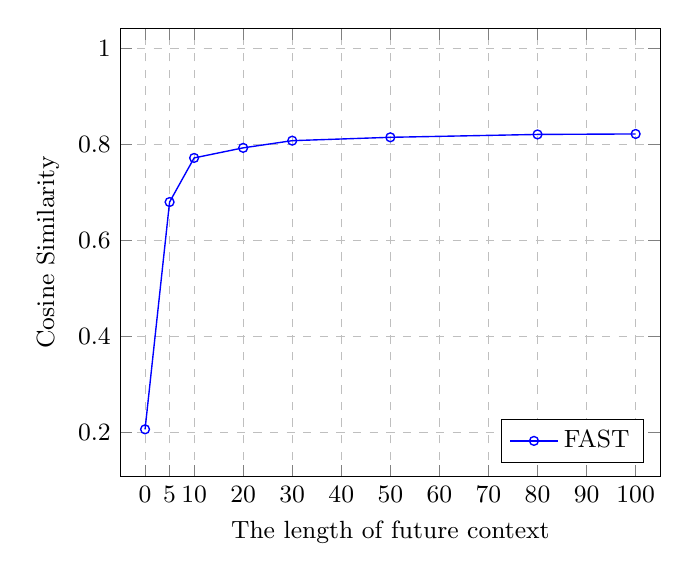
\begin{tikzpicture}[baseline]
\begin{axis}[
    ylabel=Cosine Similarity,
    xlabel=The length of future context,
    enlargelimits=0.05,
    legend pos=south east,
    legend style={font=\small},
    font=\small,
    ymajorgrids=true,
    xmajorgrids=true,
    grid style=dashed,
    ymin=0.15, ymax = 1.0,
    xtick={0,5,10,20,30,40,50,60,70,80,90,100},
]
\addplot[color=blue,mark=o, mark size=1.6pt,line width=0.5pt] coordinates{(0,0.206)(5,0.68)(10,0.772)(20,0.793)(30,0.808)(50,0.815)(80,0.821)(100,0.822)};
\legend{FAST,FAI}
\end{axis}
\end{tikzpicture}
\caption{Effect on the $\Bar{s}_{-1}$ w.r.t. $m$.}
\label{fig:length_cos}
\end{figure}

To answer this question, we explore the FAST (FAD + FAI) with different lengths of future context. 
Figure \ref{fig:length_bleu} shows the overall results. %in $\{0,10,20,30,40,50,60,70\}$
$m=0$ means the offline system without distillation. 
The offline system inherits the mismatch problem, but our method gradually improves the performance as $m$ increasing from 0 to 20. 
Since we found only the representation of last 10 positions is poor (in Section \ref{sec:analysis}), FAST obtains similar BLEU-AL curve when $m$ is significantly larger than 10, \emph{e.g.}, 20-100. 

After the FAD training, we investigate the representation of the last position (before mask tokens) by $\bar{s}_{-1}$ in Eq.~(\ref{eq:audio_cos2}) w.r.t. $m$. 
The results are shown in Figure \ref{fig:length_cos}.
We observe that 1) as $m$ increases, the streaming speech representation of the last position becomes better; 
2) the curves of the cosine similarity becomes flattened when $m > 10$ significantly. 
This is consistent with the trend in Figure \ref{fig:length_bleu}.


\subsection{Analysis on The Representation Gap}

\definecolor{poscolor4}{HTML}{38ada9}
\definecolor{poscolor5}{HTML}{78e08f}
\definecolor{poscolor6}{HTML}{b8e994}
\definecolor{poscolor7}{HTML}{008BCC}
\definecolor{poscolor8}{HTML}{00AC53}
\definecolor{poscolor9}{HTML}{3E4372}
\begin{figure}[t]
\centering
\pgfplotsset{
    width=8cm,height=5.5cm,
    every axis y label/.append style={at={(-0.1,0.5)}},
    every axis/.append style={line width=0.6pt},
}

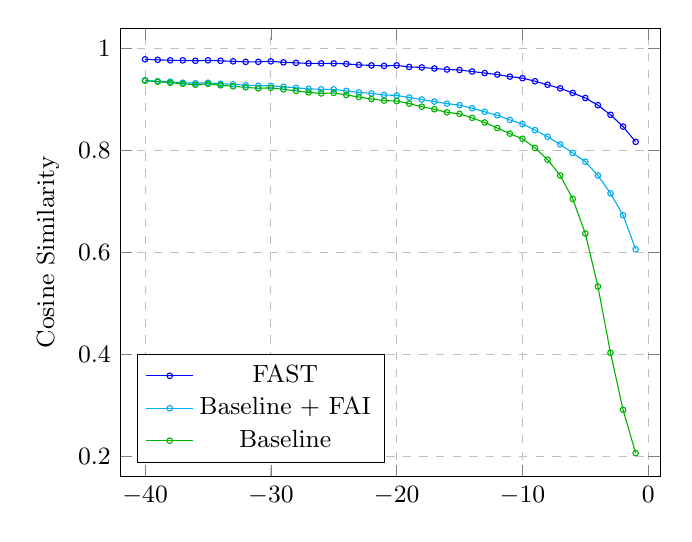
\begin{tikzpicture}[baseline]
\begin{axis}[
    ylabel=Cosine Similarity,
    enlargelimits=0.05,
    font=\small,
    legend pos=south west,
    legend style={font=\small},
    ymajorgrids=true,
    xmajorgrids=true,
    grid style=dashed,
    ymin=0.2, ymax = 1.0,
    ytick={0.2,0.4,0.6,0.8,1.0},
]
\addplot[color=blue,mark=o, mark size=1pt] coordinates{(-40,0.979)(-39,0.978)(-38,0.977)(-37,0.977)(-36,0.976)(-35,0.977)(-34,0.976)(-33,0.975)(-32,0.974)(-31,0.974)(-30,0.975)(-29,0.973)(-28,0.972)(-27,0.971)(-26,0.971)(-25,0.971)(-24,0.97)(-23,0.968)(-22,0.967)(-21,0.966)(-20,0.967)(-19,0.964)(-18,0.963)(-17,0.961)(-16,0.959)(-15,0.958)(-14,0.955)(-13,0.952)(-12,0.949)(-11,0.945)(-10,0.942)(-9,0.936)(-8,0.929)(-7,0.922)(-6,0.913)(-5,0.903)(-4,0.889)(-3,0.87)(-2,0.847)(-1,0.817)};
\addplot[color=cyan,mark=o, mark size=1pt] coordinates{(-40,0.938)(-39,0.936)(-38,0.935)(-37,0.933)(-36,0.932)(-35,0.933)(-34,0.931)(-33,0.930)(-32,0.928)(-31,0.927)(-30,0.927)(-29,0.925)(-28,0.923)(-27,0.921)(-26,0.920)(-25,0.920)(-24,0.917)(-23,0.914)(-22,0.912)(-21,0.909)(-20,0.908)(-19,0.904)(-18,0.900)(-17,0.896)(-16,0.892)(-15,0.889)(-14,0.883)(-13,0.876)(-12,0.869)(-11,0.860)(-10,0.852)(-9,0.840)(-8,0.827)(-7,0.812)(-6,0.795)(-5,0.778)(-4,0.751)(-3,0.716)(-2,0.673)(-1,0.606)};
\addplot[color=green!70!black,mark=o, mark size=1pt] coordinates{(-40,0.937)(-39,0.935)(-38,0.933)(-37,0.931)(-36,0.929)(-35,0.931)(-34,0.928)(-33,0.926)(-32,0.924)(-31,0.922)(-30,0.923)(-29,0.920)(-28,0.917)(-27,0.914)(-26,0.912)(-25,0.913)(-24,0.909)(-23,0.905)(-22,0.901)(-21,0.898)(-20,0.897)(-19,0.892)(-18,0.886)(-17,0.881)(-16,0.875)(-15,0.872)(-14,0.864)(-13,0.855)(-12,0.844)(-11,0.833)(-10,0.823)(-9,0.805)(-8,0.782)(-7,0.751)(-6,0.705)(-5,0.637)(-4,0.533)(-3,0.403)(-2,0.291)(-1,0.206)};
\legend{FAST,Baseline + FAI,Baseline,}
\end{axis}
\end{tikzpicture}
\caption{Effect on the average cosine similarity $\Bar{s}_{-t^{\prime}}$ of the streaming speech representations at the end positions (before mask tokens). After applying FAI and FAST, the representations of the end positions are improved.}
\label{fig:whywork}
\end{figure}











Figure \ref{fig:whywork} plots the changes of average cosine similarity $\Bar{s}_{-t^{\prime}}$ in Eq.~(\ref{eq:audio_cos2}) of the last 40 positions (before mask tokens) in the streaming speech after applying the FAI or FAST (FAD + FAI). 
They achieve at least 0.6 and 0.8 cosine similarity at the last position, respectively. 
The baseline only has the $<0.6$ cosine similarity for the last 4 positions and only 0.2 for the last position. 
It indicates that the representations with FAI are closer to those of the full speech, especially at the ending positions, and FAD training can further close this gap. 


\subsection{What examples are improved?}
\label{sec:monotonic}
\begin{table*}[t]

\begin{center}
\begin{tabular}{l|l|l|l|c}
\toprule
Monotonic Level & \multicolumn{1}{c|}{\textbf{Easy}}  & \multicolumn{1}{c|}{\textbf{Medium}} & \multicolumn{1}{c|}{\textbf{Hard}}  & \textbf{AL}   \\ \midrule
Offline (greedy) & 26.38 & 23.22 & 21.26 & -     \\
Baseline            & 18.88 & 12.95 & 10.38  & 1295 \\ %
+ FAI        & 23.88$^{+5.00}$ & 18.99$^{+6.04}$ & 16.45$^{+6.07}$  & 1143 \\ 
FAST         & 24.44$^{+5.56}$ & 19.89$^{+6.94}$ & 16.53$^{+6.15}$  & 1135 \\\bottomrule
\end{tabular}
\end{center}
\caption{Performance (BLEU) on different monotonic levels on test set of MuST-C EnDe.}
\label{tab:reorder}
\end{table*}

For tst-COMMON on MuST-C EnDe, we use awesome-align\footnote{\url{https://github.com/neulab/awesome-align}} \cite{dou-neubig-2021-word} to identify the token-level alignment between source transcription and target translation following \citet{zhang-feng-2022-reducing}. 
First, we define the source-to-target alignment position shift as $\max\{0, i - j\}$, where the $i$th source token is aligned to the $j$th target token. 
If $i - j$ is large, it means in order to translate the $j$th target token, the model may need to read more until seeing the $i$th source token. 
Then we calculate the monotonic level of each example as the averaged alignment position shift over the number of aligned tokens, \emph{i.e.}, 
\begin{equation}
    \mathbf{M} = \frac{1}{|\mathbf{A}|}\sum_{(i,j) \in \mathbf{A}} \max\{0, i - j\}.
\end{equation} 
where $\mathbf{M}$ denotes monotonic level and $\mathbf{A}$ represents aligned pairs.
We evenly divide the test set into three groups (Easy, Medium, and Hard) according to different monotonicity levels. %: easy ($=0$), medium ($<3$) and hard ($\geq 3$).  
For each group, we evaluate different inference methods and report the results in Table \ref{tab:reorder}. 
As we explained in \ref{apd:al}, it is almost impossible to guarantee the same AL for different inference methods. 
For a fair comparison, we try our best to set the AL of different methods to be approximately equal. 
We can see our inference strategies show a significant advantage on the non-monotonic examples (Medium and Hard groups). 



\section{Conclusion}
In this paper, we examine streaming speech translation from a new perspective. 
We investigate the effects of the input mismatch between offline-training and online-decoding.
We find that the representations at the ending positions in the streaming input are particularly poor, directly impacting the translation quality.
We propose FAST, which introduces future contexts to improve these representations during training and testing via FAD and FAI, respectively.
Experiments and analysis demonstrate their effectiveness in bridging the representation gap between full speech encoding and partial streaming encoding. 
Furthermore, our methods can be generally beneficial to streaming speech translation models that are based on Wav2Vec2.0. 
In the future, we will explore the relevant method independent on Wav2Vec2.0.



% \section*{Acknowledgements}


% Entries for the entire Anthology, followed by custom entries
\bibliography{anthology,custom}

\newpage
\appendix
% \onecolumn

\input{algos/fai.tex}

\section{Data Statistics}
\label{apd:data_statistics}
We evaluate our model on MuST-C V1 English-German (EnDe), English-Spanish (EnEs) and English-French (EnFr) datasets \citep{di-gangi-etal-2019-must}.
For training set, we follow \citet{dong-etal-2022-learning} to filter out short speech of less than 1000 frames (62.5ms) and long speech of more than 480,000 frames (30s).
The statistics of different language pairs are illustrated in Table \ref{tab:data_statistics}.
\begin{table*}
    \begin{minipage}[t]{0.19\linewidth}
        \vspace{0pt}
        \centering
        \includegraphics[width=0.98\linewidth]{sec/image/color.pdf}
        \captionsetup{font={small}}
        \figcaption{\textbf{Color contrast.} Our synthetic data shows a similar distribution of {color contrast} with real-world dataset DUTS-TR.}
        \label{fig:color}
    \end{minipage}\hspace{5pt}
    \begin{minipage}[t]{0.19\linewidth}
        \vspace{0pt}
        \centering
        \includegraphics[width=0.98\linewidth]{sec/image/size.pdf}
        \captionsetup{font={small}}
        \figcaption{\textbf{Object size.} 
        Our synthetic data has a broader scale of salient objects (object sizes ranging from $0.1$ to $0.5$).
        }
        \label{fig:size}
    \end{minipage}\hspace{5pt}
    \begin{minipage}[t]{0.37\linewidth}
            \vspace{0pt}
            \includegraphics[width=.48\linewidth]{sec/image/ours_point.pdf}
            \includegraphics[width=.48\linewidth]{sec/image/duts_tr_point.pdf}
            \figcaption{\textbf{Center bias scatter plot for our synthetic dataset (left) and DUTS-TR (right).} DUTS-TR is object-centric, while our dataset is more diverse in center distribution and contains more hard samples.}
            \label{fig:center_bias}
    \end{minipage}\hspace{5pt}
    \begin{minipage}[t]{0.19\linewidth}
        \vspace{0pt}
        \resizebox{.98\textwidth}{!}{
          \begin{tabular}{c|cc}
            \toprule
            &DUTS-TR&Ours\\\midrule
            SC&27.1&29.9\\\midrule
            PL&2.96&2.78\\\midrule
            SD&2.31&1.91\\
            \bottomrule
          \end{tabular}
        }
        \tabcaption{\textbf{Geometry statistics,} in terms of shape complexity (SC), polygon length (PL) and shape diversity (SD). 
        }
        \label{tab:shape}
      \end{minipage}
\end{table*}





\section{Additional Preliminary Analysis}
\label{apd:additional_analysis}

\subsection{Which part of streaming speech representation is worse?}
\label{sec:which_part}
To further verify that only the representation of the end position in streaming speech is poor,
we calculate the cosine similarity $s_{t,t^{\prime}}$ between the speech representation at the $t^{\prime}$-th ($t^{\prime} \leq t$) position in the $t$-th streaming audio input $\mathbf{\hat{x}}_t$ and the speech representation at the same position in the full encoding. 
Then we average the cosine similarities over the sentences in dataset $\mathcal{B}$ to obtain robust statistics. 
%
\begin{equation}
\begin{aligned}
\text{For $t^\prime \leq t$}, \ \Bar{s}_{t,t^{\prime}} &= \frac{1}{|\mathcal{B}_t|}\sum\limits_{\mathbf{x}\in\mathcal{B}_t} s_{t,t^\prime} (\mathbf{x}) \\
&= \frac{1}{|\mathcal{B}_t|}\sum\limits_{\mathbf{x}\in\mathcal{B}_t} \operatorname{cos}(\hat{a}_{t,t^{\prime}}, a_{t^{\prime}}), 
\label{eq:audio_cos1}
\end{aligned}
\end{equation} 
%
where $\mathcal{B}_t = \{\mathbf{x}: | \mathbf{x} | \geq t\}$ contains the audio inputs with length no shorter than $t$.

We empirically compare the averaged cosine similarity at the beginning, middle, and end positions of the speech representations. 
%The data set used for this purpose is the EnDe tst-COMMON set.
Figure \ref{fig:part} shows $\Bar{s}_{t,t^{\prime}}$ of the first three ($t^{\prime}=1,2,3$), middle three ($t^{\prime}=\lfloor \frac{1+t}{2} \rfloor-1, \lfloor \frac{1+t}{2} \rfloor, \lfloor \frac{1+t}{2} \rfloor + 1$), and last three ($t^{\prime}=t-2, t-1, t$) positions for each encoding step $t$. 
At the beginning and middle positions, the averaged cosine similarity $\Bar{s}_{t,t^{\prime}}$ is greater than 0.8 except $t^\prime=1$, indicating that the representations at such positions in the partial streaming input are close to those in the full speech. 
Note that $t^\prime=1$ with a slightly lower similarity won't hurt the performance much, because in practice it is almost impossible to apply \textit{wait}-1 policy (only read 20\emph{ms} speech input) in streaming ST. 
However, the $\Bar{s}_{t,t^{\prime}}$ declines significantly for the end positions, especially for the last one. 
In addition, we observe that as $t$ becomes larger, the streaming input will gradually approximate the full speech input, then the gap of the speech representation between the offline and the online input becomes smaller. 
We conclude that \textbf{the representations of the end position in the streaming speech are particularly inferior.}
\begin{figure*}[t]
\centering
\subfigure[$\Bar{s}_{t,t^{\prime}}$ of the first three positions]{
\includegraphics[width=0.32\linewidth]{figs/csv_files/part_cos_first.eps}
}
~
\subfigure[$\Bar{s}_{t,t^{\prime}}$ of middle three positions]{
\includegraphics[width=0.3\linewidth]{figs/csv_files/part_cos_mid.eps}
}
~
\subfigure[$\Bar{s}_{t,t^{\prime}}$ of the last three positions]{
\includegraphics[width=0.3\linewidth]{figs/csv_files/part_cos_end.eps}
}
\caption{The average cosine similarity $\Bar{s}_{t,t^{\prime}}$ of the first three ($t^{\prime}=1,2,3$), middle three ($t^{\prime}=\lfloor \frac{1+t}{2} \rfloor-1, \lfloor \frac{1+t}{2} \rfloor, \lfloor \frac{1+t}{2} \rfloor + 1$), and last three ($t^{\prime}=t-2,t-1,t$) positions for each encoding step $t$.}
\label{fig:part}
\end{figure*}








\begin{figure}[t]
\centering
\pgfplotsset{
    width=7.5cm,height=5.5cm,
    every axis y label/.append style={at={(-0.09,0.5)}},
    every axis/.append style={line width=0.4pt},
}
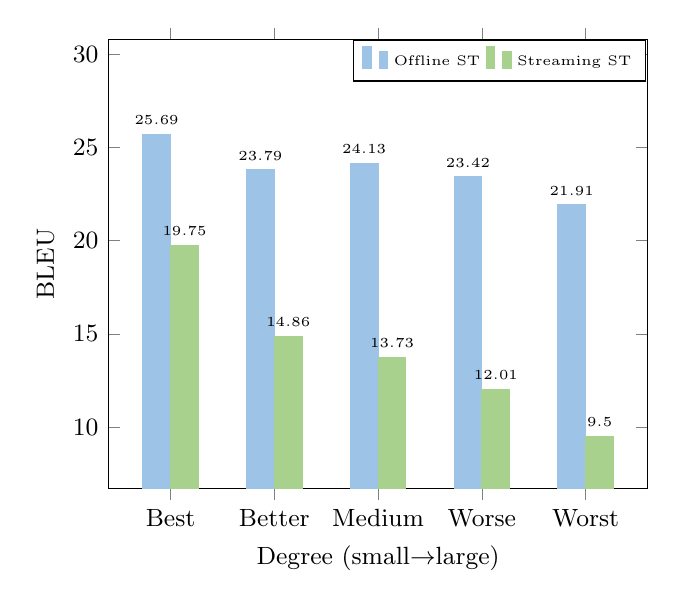
\begin{tikzpicture}[baseline]
\begin{axis}[
    legend style={at={(0.725,1)},
    anchor=north,
    legend columns=2,
    font=\tiny},
    enlargelimits=0.15, 
    font=\small,
    ylabel={BLEU},
    xlabel={Degree (small$\rightarrow$large)},
    xtick=data,
    symbolic x coords={Best,Better,Medium,Worse,Worst},
    xticklabel style={name=tick no\ticknum},
    bar width=10pt,
    nodes near coords,
    nodes near coords align={vertical},
    nodes near coords style={font=\tiny},
    ymax=28,
    ybar=0.1pt,
]

\addplot[ybar, draw=blue1, fill=blue1]
    coordinates {(Best,25.69)(Better,23.79)(Medium,24.13)(Worse,23.42)(Worst,21.91)};

\addplot[ybar, draw=green2, fill=green2]
    coordinates {(Best,19.75)(Better,14.86)(Medium,13.73)(Worse,12.01)(Worst,9.50)};
\legend{Offline ST,Streaming ST}

\end{axis}
\end{tikzpicture}
\caption{Performance with degree of deterioration of the representation at the last position of the streaming speech.}
\label{fig:degree}
\end{figure}

\subsection{Does the poor representation at the last positions of streaming speech affect streaming ST performance?}
\label{apd:degree}



To answer this question, we only calculate the average cosine similarity in the last position for each sample. 
%
\begin{equation}
\forall \mathbf{x}, \quad \Bar{s}_{-1} (\mathbf{x})= \frac{1}{T}\sum\limits_{t=1}^{t=T} \operatorname{cos}(\hat{a}_{t,t}, a_{t}),
\label{eq:audio_cos3}
\end{equation}
%
$\Bar{s}_{-1}(\mathbf{x})$ reflects the degree of deterioration of the representation at the last position of the streaming speech. 
We sort the dataset by the value of the degree and divide them evenly into 5 groups to ensure enough samples in each group. The translation quality of each group is shown in Figure \ref{fig:degree}. 
The performance of streaming ST drops close to 10 points as the representation at the last position of the streaming speech becomes worse, while the full-sentence ST fluctuates less than 4 points. 
In addition, the performance gap between the streaming ST and the full-sentence ST becomes larger as the representation at the last position gets worse. In the worse group, the streaming ST is 12.41 points lower than the full-sentence ST. 
Therefore, we conclude that \textbf{the poor representation at the end position of the streaming speech has a strong effect on the translation quality.} 


\section{Details of Offline Training} 
\label{apd:details_of_training} 

We use an Adam optimizer with learning rate $1e^{-4}$ and warmup step $10k$.
We decay the learning rate with inverse square root schedule. 

The offline ST model is first trained by a multi-task learning, including ASR and ST tasks. 
A language identity tag is prepended to the target sentence for indicating which task is learned. 
In this stage, the CIF module which is used to detect the acoustic boundary is deactivated, in other words, the CIF module is not trained. 
The main purpose is to learn a better decoder, i.e., a well-trained language model. 
Then, we activate the CIF module such that its parameters are trainable, and continue to train for another several epochs. 
In this stage, only the ST task is learned. 


\section{Additional Experiments}

\subsection{Why we use AL rather than \textit{k}?}
\label{apd:al}

In our presented results, we plot the BLEU \emph{v.s.} AL rather than $k$. 
We argue that $k$ is not a fair metric to evaluate the latency. 
In text streaming translation, different tokenization (\emph{e.g.}, different number of BPE operations) will lead to different token boundaries for the same sentence. 
It indicates the $k$ tokens do not necessarily represent the same partial sentence for different BPE methods. 
This situation becomes even severer for speech streaming translation. 
As we have a source text token boundary detector in our model, the first $k$ detected text tokens will represent different lengths of audio frames for different input audios. 
To be precise, the wait-$k$ policy used in our streaming speech translation is actually wait-$k$ detected tokens policy. 
Therefore, we prefer to use AL rather than $k$ as the latency metric in our experiments. 



\subsection{How important of the Wav2Vec2.0?}
\label{apd:w2v2}

\begin{figure*}[t]
\pgfplotsset{width=8cm,height=5.5cm,
    every axis y label/.append style={at={(-0.1,0.5)}},
    every axis/.append style={line width=0.6pt},
}
\centering
\subfigure[MuST-C]{
\begin{tikzpicture}[baseline]
\begin{axis}[
    ylabel=Cosine Similarity,
    xlabel=Distance from consumed speech,
    enlargelimits=0.05,
    legend pos=north east,
    legend style={font=\small},
    ymajorgrids=true,
    xmajorgrids=true,
    grid style=dashed,
    font=\small,
    xtick={-10,0,10,20,30,40},
]
\addplot[color=red,mark=o, mark size=0.8pt,line width=0.6pt] coordinates{(-10,0.852)(-9,0.840)(-8,0.827)(-7,0.812)(-6,0.795)(-5,0.778)(-4,0.751)(-3,0.716)(-2,0.673)(-1,0.606)(0,0.568)(1,0.509)(2,0.462)(3,0.422)(4,0.382)(5,0.347)(6,0.319)(7,0.294)(8,0.272)(9,0.254)(10,0.239)(11,0.227)(12,0.217)(13,0.208)(14,0.201)(15,0.195)(16,0.190)(17,0.187)(18,0.183)(19,0.180)(20,0.176)(21,0.173)(22,0.170)(23,0.166)(24,0.162)(25,0.158)(26,0.154)(27,0.150)(28,0.146)(29,0.141)(30,0.137)(31,0.132)(32,0.128)(33,0.124)(34,0.123)(35,0.123)(36,0.123)(37,0.123)(38,0.122)(39,0.119)(40,0.116)(41,0.111)(42,0.106)(43,0.102)(44,0.100)(45,0.117)(46,0.125)(47,0.126)(48,0.127)(49,0.126)};
\addplot[color=poscolor7,mark=o, mark size=0.8pt] coordinates{(-10,0.681)(-9,0.680)(-8,0.676)(-7,0.672)(-6,0.668)(-5,0.665)(-4,0.661)(-3,0.648)(-2,0.596)(-1,0.466)(0,0.354)(1,0.269)(2,0.220)(3,0.183)(4,0.150)(5,0.122)(6,0.099)(7,0.084)(8,0.074)(9,0.068)(10,0.067)(11,0.068)(12,0.069)(13,0.071)(14,0.072)(15,0.072)(16,0.070)(17,0.068)(18,0.065)(19,0.062)(20,0.060)(21,0.060)(22,0.060)(23,0.059)(24,0.058)(25,0.051)(26,0.050)(27,0.049)(28,0.049)(29,0.049)(30,0.050)(31,0.050)(32,0.050)(33,0.048)(34,0.045)(35,0.041)(36,0.037)(37,0.032)(38,0.027)(39,0.025)(40,0.024)(41,0.024)(42,0.026)(43,0.028)(44,0.031)(45,0.031)(46,0.030)(47,0.028)(48,0.022)(49,0.014)}; 
\legend{finetuned-w2v2,pretrained-w2v2}
\end{axis}
\end{tikzpicture}}
~~~
\subfigure[LibriSpeech]{
\begin{tikzpicture}[baseline]
\begin{axis}[
    ylabel=Cosine Similarity,
    xlabel=Distance from consumed speech,
    enlargelimits=0.05,
    legend pos=north east,
    legend style={font=\small},
    ymajorgrids=true,
    xmajorgrids=true,
    grid style=dashed,
    font=\small,
    xtick={-10,0,10,20,30,40},
]
\addplot[color=red,mark=o, mark size=0.8pt] coordinates{(-10,0.8470)(-9,0.836)(-8,0.823)(-7,0.809)(-6,0.793)(-5,0.775)(-4,0.751)(-3,0.719)(-2,0.677)(-1,0.61)(0,0.572)(1,0.516)(2,0.474)(3,0.436)(4,0.399)(5,0.366)(6,0.339)(7,0.315)(8,0.293)(9,0.274)(10,0.258)(11,0.245)(12,0.233)(13,0.222)(14,0.213)(15,0.206)(16,0.200)(17,0.194)(18,0.190)(19,0.185)(20,0.181)(21,0.177)(22,0.173)(23,0.169)(24,0.166)(25,0.162)(26,0.158)(27,0.155)(28,0.151)(29,0.148)(30,0.144)(31,0.141)(32,0.139)(33,0.136)(34,0.136)(35,0.136)(36,0.136)(37,0.135)(38,0.134)(39,0.131)(40,0.130)(41,0.128)(42,0.126)(43,0.124)(44,0.121)(45,0.117)(46,0.115)(47,0.114)(48,0.116)(49,0.114)}; 
\addplot[color=poscolor7,mark=o, mark size=0.8pt] coordinates{(-10,0.639)(-9,0.635)(-8,0.631)(-7,0.626)(-6,0.620)(-5,0.616)(-4,0.606)(-3,0.582)(-2,0.495)(-1,0.351)(0,0.236)(1,0.170)(2,0.138)(3,0.113)(4,0.092)(5,0.072)(6,0.055)(7,0.042)(8,0.034)(9,0.028)(10,0.025)(11,0.025)(12,0.026)(13,0.028)(14,0.030)(15,0.032)(16,0.032)(17,0.032)(18,0.031)(19,0.031)(20,0.030)(21,0.030)(22,0.030)(23,0.030)(24,0.029)(25,0.025)(26,0.024)(27,0.024)(28,0.024)(29,0.024)(30,0.024)(31,0.023)(32,0.022)(33,0.018)(34,0.012)(35,0.005)(36,-0.003)(37,-0.010)(38,-0.013)(39,-0.014)(40,-0.013)(41,-0.010)(42,-0.005)(43,-0.001)(44,0.001)(45,-0.001)(46,-0.004)(47,-0.014)(48,-0.023)(49,-0.001)}; 
\legend{finetuned-w2v2,pretrained-w2v2}
\end{axis}
\end{tikzpicture}}
\caption{We measure the accuracy of predicted context by calculating the cosine similarity between every predicted future representation and full speech representations at the same position. }
\label{fig:mask_acc}
\end{figure*}

As we mentioned in the main text, the special audio token ``mask" in Wav2Vec2.0 is pre-trained on the Librispeech dataset to reconstruct the corresponding feature conditional on unmasked context via the contrastive task. 
In our experiments, we didn't include contrastive learning as the auxiliary task in the downstream ST training. 
And in our FAI inference, we directly leverage the mask embeddings as the future context by appending them to the streaming input. 
However, we found the speech representations after ST training becomes even better. 
Particularly, we calculate the cosine similarity between every predicted future representation and full speech representations at the same position, and the results are illustrated in Figure \ref{fig:mask_acc}. 
On either the Librispeech or the MuST-C audio test set, the fine-tuned Wav2Vec2.0 can produce better speech representations from the masking inputs. 


\subsection{Why $m>10$?}
Based on the analysis in Section 3, we observed that the representations of the last 10 positions of the streaming speech are poorer. For example, the speech representations $\mathbf{\hat{a}}_{t-10:t}$ for streaming speech $\mathbf{c}_{1:t}$ of length $t$ are poor. Similarly, in FKD for a teacher's streaming speech input $\mathbf{c}_{1:t+m}$ of length $t+m$, the speech representations $\mathbf{\hat{a}}_{t+m-10:t+m}$ are always suboptimal. Hence, not all $t+m$ speech representations can be utilized as teachers, only the first $t$ speech representations are taken into account for loss calculation. If $m < 10$, $t+m-10$ will be smaller than $t$, and the representations $\mathbf{\hat{a}}_{t-10+m:t}$ will also be of inferior quality, making the representation $\mathbf{\hat{a}}_{t-10+m:t}$ a poor teacher. Thus, $m$ needs to be greater than 10 for high quality teachers.





\subsection{Why are all predicted features discarded?}
\label{apd:discard}
\begin{figure}[t]

\pgfplotsset{width=7.5cm,height=5.5cm,
    every axis y label/.append style={at={(-0.12,0.5)}},
    every axis/.append style={line width=0.6pt},
}
\centering
\begin{tikzpicture}[baseline]
\begin{axis}[
    ylabel=BLEU,
    xlabel=Average Lagging(ms),
    enlargelimits=0.05,
    legend pos=south east,
    legend columns=1,
    legend style={font=\small},
    font=\small,
    xmajorgrids=true,
    ymajorgrids=true,
    grid style=dashed,
    ytick={4,8,12,16,20,24},
]
\addplot[color=poscolor7,mark=o, line width=0.6pt, mark size=1.8pt] coordinates {(475.48,12.65)(795.84,16.1)(1143.37,19.19)(1533.63,21.15)(2109.41,22.23)(2647.03,23.15)(3403.9,23.65)}; 
\addplot[color=poscolor8,mark=o, line width=0.6pt, mark size=1.8pt] coordinates {(615.63,9.77)(927.32,14.99)(1304.13,18.63)(1897.08,21.59)(2457.97,22.76)(3269.3,23.32)};
\addplot[color=teal,mark=o, line width=0.6pt, mark size=1.8pt] coordinates {(374.32,1.78)(931.56,8.3)(1326.92,14.92)(1717.09,20.27)(2298.95,22.23)(3155.64,23.26)};
\addplot[color=olive,mark=o, line width=0.6pt, mark size=1.8pt] coordinates {(581.74,0.96)(1218.34,4.26)(1885.57,11.25)(2288.62,16.96)(2546.59,21.59)(3170.2,23.07)};
\legend{$p=1.0$,$p=0.8$,$p=0.4$,$p=0.0$}
\end{axis}
\end{tikzpicture}
\caption{BLEU \emph{v.s.} AL on different $p$.}
\label{fig:discard}
\end{figure}

In FAI strategy, all the output representations corresponding to the $m=50$ masking tokens will be discarded, because we have demonstrated that the representations at the ending positions are inferior. 
However, as shown in \ref{fig:mask_acc}, the first 10 predicted representations are not as bad as the next 40. 
Therefore, on the EnDE test set, we also conduct another streaming ST inference by appending different numbers of predicted context to the original speech representations. 
We use discard rate $p$ to measure the number of appending features. 
When $p=1.0$, all predicted features are discarded and it reduces to the standard FAI inference. 
In Figure \ref{fig:discard}, we compare the streaming speech translation quality between regular FAI and its variant. 
It is concluded that the predicted future context is too noisy and harmful to the performance.


\subsection{Additional Results on EnDe/Es and EnFr}
\label{apd:appendix_more_results}

In this section, we evaluate our methods with other latency metrics AP and DAL. 
The AP-BLEU and DAL-BLEU curves on the MuST-C EnDe, EnEs, and EnFr tst-COMMON sets are shown in Figure \ref{fig:expand_results}. 
For three language pairs, our methods can consistently improve the baseline by a large margin. 

\begin{figure*}[!tbp]
\pgfplotsset{width=7.5cm,height=5.8cm,
    every axis y label/.append style={at={(-0.1,0.5)}},
    every axis/.append style={line width=0.6pt},
}
\centering
\subfigure[EnDe]{
\begin{tikzpicture}[baseline]
\begin{axis}[
    ylabel=BLEU,
    xlabel=Average Proportion,
    enlargelimits=0.04,
    font=\small,
    legend pos=south east,
    legend style={font=\scriptsize},
    xmajorgrids=true,
    ymajorgrids=true,
    grid style=dashed,
    ytick={0,4,8,12,16,20,24},
]
\addplot[color=black,dashed,line width=0.8pt] coordinates {(0.1,23.53)(1,23.53)};
\addplot[color=maincolor,mark=*, mark size=1.8pt] coordinates {(0.13,0.02)(0.32,1.68)(0.51,7.79)(0.65,13.31)(0.78,18.72)(0.85,20.67)(0.92,22.33)(0.97,23.16)(1.0,23.29)}; 
\addplot[color=maincolor2,mark=*, mark size=1.8pt,line width=0.8pt] coordinates {(0.3,5.94)(0.53,12.65)(0.63,16.1)(0.7,19.19)(0.76,21.15)(0.83,22.23)(0.88,23.15)(0.93,23.65)(0.97,23.42)};
\addplot[color=maincolor3,mark=*, mark size=1.8pt,line width=0.8pt] coordinates {(0.54,12.69)(0.61,14.78)(0.67,17.71)(0.73,19.67)(0.78,21.36)(0.83,22.51)(0.88,22.84)(0.92,23.36)(0.97,23.55)};

\legend{offline (greedy),Baseline (\textbf{B}),\textbf{B} + FAI,\textbf{B} + FAD + FAI (\textbf{FAST})}
\end{axis}
\end{tikzpicture}}
~
\subfigure[EnDe]{
\begin{tikzpicture}[baseline]
\begin{axis}[
    xlabel=Differentiable Average Lagging,
    enlargelimits=0.04,
    font=\small,
    legend pos=south east,
    legend style={font=\scriptsize},
    xmajorgrids=true,
    ymajorgrids=true,
    grid style=dashed,
    ytick={0,4,8,12,16,20,24},
]
\addplot[color=black,dashed,line width=0.8pt] coordinates {(360,23.53)(6000,23.53)};
\addplot[color=maincolor,mark=*, mark size=1.8pt] coordinates {(359,0.02)(656,1.68)(1032,7.79)(1531,13.31)(2234,18.72)(2788,20.67)(3559,22.33)(4576,23.16)(5791,23.29)}; 
\addplot[color=maincolor2,mark=*, mark size=1.8pt,line width=0.8pt] coordinates {(494,5.94)(928,12.65)(1223,16.1)(1559,19.19)(1928,21.15)(2476,22.23)(2974,23.15)(3678,23.65)(4625,23.42)}; 
\addplot[color=maincolor3,mark=*, mark size=1.8pt,line width=0.8pt] coordinates {(731,12.69)(1009,14.78)(1327,17.71)(1655,19.67)(1991,21.36)(2483,22.51)(2932,22.84)(3581,23.36)(4510,23.55)}; 

\legend{offline (greedy),Baseline (\textbf{B}),\textbf{B} + FAI,\textbf{B} + FAD + FAI (\textbf{FAST})}
\end{axis}
\end{tikzpicture}}
~
\subfigure[EnEs]{
\begin{tikzpicture}[baseline]
\begin{axis}[
    ylabel=BLEU,
    xlabel=Average Proportion,
    enlargelimits=0.04,
    font=\small,
    legend pos=south east,
    legend style={font=\scriptsize},
    xmajorgrids=true,
    ymajorgrids=true,
    grid style=dashed,
    ytick={0,4,8,12,16,20,24,28},
]
\addplot[color=black,dashed,line width=0.8pt] coordinates {(0.34,27.81)(1,27.81)};
\addplot[color=maincolor,mark=*, mark size=1.8pt] coordinates {(0.34,2.39)(0.4,4.09)(0.55,11.37)(0.7,20.31)(0.79,24.62)(0.87,27.04)(0.91,27.74)(0.96,27.88)(0.99,27.76)}; 
\addplot[color=maincolor2,mark=*, mark size=1.8pt,line width=0.8pt] coordinates {(0.35,8.38)(0.59,17.86)(0.7,22.71)(0.78,25.92)(0.83,27.15)(0.89,27.8)(0.93,28.04)(0.96,27.88)(0.99,27.71)};
\addplot[color=maincolor3,mark=*, mark size=1.8pt,line width=0.8pt] coordinates {(0.58,18.34)(0.65,21.53)(0.73,24.78)(0.79,26.4)(0.84,27.24)(0.89,28.02)(0.92,27.98)(0.96,28.23)(0.98,28.09)};
\legend{offline (greedy),Baseline (\textbf{B}),\textbf{B} + FAI,\textbf{B} + FAD + FAI (\textbf{FAST})}
\end{axis}
\end{tikzpicture}}
~
\subfigure[EnEs]{
\begin{tikzpicture}[baseline]
\begin{axis}[
    xlabel=Differentiable Average Lagging,
    enlargelimits=0.04,
    font=\small,
    legend pos=south east,
    legend style={font=\scriptsize},
    xmajorgrids=true,
    ymajorgrids=true,
    grid style=dashed,
    ytick={4,8,12,16,20,24,28},
]
\addplot[color=black,dashed,line width=0.8pt] coordinates {(640,27.81)(4500,27.81)};
\addplot[color=maincolor,mark=*, mark size=1.8pt] coordinates {(1007,2.39)(1054,4.09)(1239,11.37)(1700,20.31)(2215,24.62)(2947,27.04)(3513,27.74)(4260,27.88)(5157,27.76)}; 
\addplot[color=maincolor2,mark=*, mark size=1.8pt,line width=0.8pt] coordinates {(641,8.38)(1181,17.86)(1589,22.71)(2037,25.92)(2500,27.15)(3114,27.8)(3630,28.04)(4328,27.88)(5181,27.71)}; 
\addplot[color=maincolor3,mark=*, mark size=1.8pt,line width=0.8pt] coordinates {(860,18.34)(1232,21.53)(1629,24.78)(2056,26.4)(2471,27.24)(3040,28.02)(3550,27.98)(4214,28.23)(5082,28.09)}; 
\legend{offline (greedy),Baseline (\textbf{B}),\textbf{B} + FAI,\textbf{B} + FAD + FAI (\textbf{FAST})}
\end{axis}
\end{tikzpicture}}
~
\subfigure[EnFr]{
\label{fig:en-fr-ap}
\begin{tikzpicture}[baseline]
\begin{axis}[
    ylabel=BLEU,
    xlabel=Average Proportion,
    enlargelimits=0.04,
    font=\small,
    legend pos=south east,
    legend style={font=\scriptsize},
    xmajorgrids=true,
    ymajorgrids=true,
    grid style=dashed,
    ytick={6,12,18,24,30},
]
\addplot[color=black,dashed,line width=0.6pt] coordinates {(0.35,33.63)(0.95,33.63)};
\addplot[color=maincolor,mark=*, mark size=1.8pt] coordinates {(0.35,3.27)(0.38,3.62)(0.46,6.95)(0.59,15.1)(0.69,21.66)(0.79,27.4)(0.86,29.89)(0.92,31.7)(0.97,33.09)}; 
\addplot[color=maincolor2,mark=*, mark size=1.8pt,line width=0.6pt] coordinates {(0.44,14.45)(0.54,17.61)(0.61,20.63)(0.69,25.87)(0.76,28.95)(0.83,31.47)(0.88,32.68)(0.93,33.11)(0.97,33.54)};
\addplot[color=maincolor3,mark=*, mark size=1.8pt,line width=0.6pt] coordinates {(0.54,19.15)(0.6,22.31)(0.67,25.78)(0.73,28.7)(0.78,30.45)(0.84,32.35)(0.88,33.03)(0.92,33.77)(0.97,33.99)}; 

\legend{offline (greedy),Baseline (\textbf{B}),\textbf{B} + FAI,\textbf{B} + FAD + FAI (\textbf{FAST})}
\end{axis}
\end{tikzpicture}}
~
\subfigure[EnFr]{
\label{fig:en-fr-dal}
\begin{tikzpicture}[baseline]
\begin{axis}[
    xlabel=Differentiable Average Lagging,
    enlargelimits=0.04,
    font=\small,
    legend pos=south east,
    legend style={font=\scriptsize},
    xmajorgrids=true,
    ymajorgrids=true,
    grid style=dashed,
    ytick={6,12,18,24,30},
]
\addplot[color=black,dashed,line width=0.6pt] coordinates {(630,33.63)(4100,33.63)};
\addplot[color=maincolor,mark=*, mark size=1.8pt] coordinates {(997,3.27)(1016,3.62)(1092,6.95)(1300,15.1)(1630,21.66)(2222,27.4)(2741,29.89)(3462,31.7)(4435,33.09)};
\addplot[color=maincolor2,mark=*, mark size=1.8pt,line width=0.6pt] coordinates {(632,14.45)(852,17.61)(1127,20.63)(1456,25.87)(1810,28.95)(2362,31.47)(2838,32.68)(3515,33.11)(4454,33.54)};
\addplot[color=maincolor3,mark=*, mark size=1.8pt,line width=0.6pt] coordinates {(705,19.15)(985,22.31)(1293,25.78)(1616,28.7)(1943,30.45)(2418,32.35)(2850,33.03)(3473,33.77)(4376,33.99)};

\legend{offline (greedy),Baseline (\textbf{B}),\textbf{B} + FAI,\textbf{B} + FAD + FAI (\textbf{FAST})}
\end{axis}
\end{tikzpicture}}
\caption{The translation quality (BLEU) against the latency metrics (AP, DAL) on the tst-COMMON set of MuST-C EnDe, EnEs and EnFr dataset.}
\label{fig:expand_results}
\end{figure*}







\section{Numeric Results for the Figures}
\label{apd:appendix_numeric_results}

\begin{table*}[!ht]
\begin{center}
\renewcommand\arraystretch{1.2}
\resizebox{\textwidth}{!}{
\begin{tabular}{lccccccccccccc}
\toprule
\multirow{2}{*}{Model}    & \multirow{2}{*}{Lagging ($k$)} & \multicolumn{4}{c}{En-De}  & \multicolumn{4}{c}{En-Es}  & \multicolumn{4}{c}{En-Fr}  \\ \cmidrule(lr){3-6} \cmidrule(lr){7-10}\cmidrule(lr){11-14}
                          &                              & AL   & AP   & DAL  & BLEU  & AL   & AP   & DAL  & BLEU  & AL   & AP   & DAL  & BLEU  \\ \cmidrule(lr){1-1} \cmidrule(lr){2-2} \cmidrule(lr){3-6} \cmidrule(lr){7-10}\cmidrule(lr){11-14}
\multirow{9}{*}{Baseline} & 1                            & 178  & 0.13 & 359  & 0.02  & 295  & 0.34 & 1007 & 2.39  & 288  & 0.35 & 997  & 3.27  \\
                          & 3                            & 483  & 0.32 & 656  & 1.68  & 543  & 0.40  & 1054 & 4.09  & 463  & 0.38 & 1016 & 3.62  \\
                          & 5                            & 659  & 0.42 & 821  & 4.34  & 882  & 0.55 & 1239 & 11.37 & 693  & 0.46 & 1092 & 6.95  \\
                          & 7                            & 867  & 0.51 & 1032 & 7.79  & 1361 & 0.70  & 1700 & 20.31 & 1028 & 0.59 & 1300 & 15.10  \\
                          & 9                            & 1295 & 0.65 & 1531 & 13.31 & 1848 & 0.79 & 2215 & 24.62 & 1406 & 0.69 & 1630 & 21.66 \\
                          & 12                           & 1939 & 0.78 & 2234 & 18.72 & 2572 & 0.87 & 2947 & 27.04 & 1972 & 0.79 & 2222 & 27.40  \\
                          & 15                           & 2505 & 0.85 & 2788 & 20.67 & 3171 & 0.91 & 3513 & 27.74 & 2495 & 0.86 & 2741 & 29.89 \\
                          & 20                           & 3312 & 0.92 & 3559 & 22.33 & 3988 & 0.96 & 4260 & 27.88 & 3245 & 0.92 & 3462 & 31.70  \\
                          & 30                           & 4410 & 0.97 & 4576 & 23.16 & 5012 & 0.99 & 5157 & 27.76 & 4283 & 0.97 & 4435 & 33.09 \\ \cmidrule(lr){1-1} \cmidrule(lr){2-2} \cmidrule(lr){3-6} \cmidrule(lr){7-10}\cmidrule(lr){11-14}
\multirow{9}{*}{+ FAI}      & 1                            & 150  & 0.30  & 494  & 5.94  & 347  & 0.35 & 641  & 8.38  & 285  & 0.44 & 632  & 14.45 \\
                          & 3                            & 475  & 0.53 & 928  & 12.65 & 775  & 0.59 & 1181 & 17.86 & 505  & 0.54 & 852  & 17.61 \\
                          & 5                            & 796  & 0.63 & 1223 & 16.10  & 1162 & 0.70  & 1589 & 22.71 & 805  & 0.61 & 1127 & 20.63 \\
                          & 7                            & 1143 & 0.70  & 1559 & 19.19 & 1608 & 0.78 & 2037 & 25.92 & 1154 & 0.69 & 1456 & 25.87 \\
                          & 9                            & 1534 & 0.76 & 1928 & 21.15 & 2076 & 0.83 & 2500 & 27.15 & 1498 & 0.76 & 1810 & 28.95 \\
                          & 12                           & 2109 & 0.83 & 2476 & 22.23 & 2736 & 0.89 & 3114 & 27.80  & 2060 & 0.83 & 2362 & 31.47 \\
                          & 15                           & 2647 & 0.88 & 2974 & 23.15 & 3301 & 0.93 & 3630 & 28.04 & 2559 & 0.88 & 2838 & 32.68 \\
                          & 20                           & 3404 & 0.93 & 3678 & 23.65 & 4072 & 0.96 & 4328 & 27.88 & 3280 & 0.93 & 3515 & 33.11 \\
                          & 30                           & 4457 & 0.97 & 4625 & 23.42 & 5045 & 0.99 & 5181 & 27.71 & 4297 & 0.97 & 4454 & 33.54 \\ \cmidrule(lr){1-1} \cmidrule(lr){2-2} \cmidrule(lr){3-6} \cmidrule(lr){7-10}\cmidrule(lr){11-14}
\multirow{9}{*}{FAST}     & 1                            & 41   & 0.54 & 731  & 12.69 & 270  & 0.58 & 860  & 18.34 & 223  & 0.54 & 705  & 19.15 \\
                          & 3                            & 403  & 0.61 & 1009 & 14.78 & 722  & 0.65 & 1232 & 21.53 & 554  & 0.60  & 985  & 22.31 \\
                          & 5                            & 771  & 0.67 & 1327 & 17.71 & 1152 & 0.73 & 1629 & 24.78 & 895  & 0.67 & 1293 & 25.78 \\
                          & 7                            & 1135 & 0.73 & 1655 & 19.67 & 1594 & 0.79 & 2056 & 26.40  & 1224 & 0.73 & 1616 & 28.70 \\
                          & 9                            & 1503 & 0.78 & 1991 & 21.36 & 2031 & 0.84 & 2471 & 27.24 & 1570 & 0.78 & 1943 & 30.45 \\
                          & 12                           & 2036 & 0.83 & 2483 & 22.51 & 2650 & 0.89 & 3040 & 28.02 & 2079 & 0.84 & 2418 & 32.35 \\
                          & 15                           & 2539 & 0.88 & 2932 & 22.84 & 3194 & 0.92 & 3550 & 27.98 & 2541 & 0.88 & 2850 & 33.03 \\
                          & 20                           & 3260 & 0.92 & 3581 & 23.36 & 3943 & 0.96 & 4214 & 28.23 & 3212 & 0.92 & 3473 & 33.77 \\
                          & 30                           & 4305 & 0.97 & 4510 & 23.55 & 4928 & 0.98 & 5082 & 28.09 & 4199 & 0.97 & 4376 & 33.99 \\ \bottomrule
\end{tabular}}
\end{center}
\caption{Numeric results on MuST-C EnDe, EnEs, and EnFr 
tst-COMMON set (Figure \ref{fig:main_results} and \ref{fig:expand_results}). }
\label{tab:main_exp_numeric}
\end{table*}


\begin{table*}[ht]
\setlength\tabcolsep{10pt}
\begin{center}
\begin{tabular}{ccccccccc}
\toprule
\multirow{2}{*}{Lagging ($k$)} & \multicolumn{2}{c}{\textit{w/o $\mathcal{L}_{KD}^{\text{W2V2}}$}} & \multicolumn{2}{c}{\textit{w/o $\mathcal{L}_{KD}^{\text{CIF}}$}} & \multicolumn{2}{c}{\textit{w/o FAI}} & \multicolumn{2}{c}{\textit{w/o mask embeds}} \\ \cmidrule(lr){2-3} \cmidrule(lr){4-5} \cmidrule(lr){6-7}\cmidrule(lr){8-9}
                               & AL         & BLEU       & AL         & BLEU       & AL         & BLEU       & AL         & BLEU        \\ \cmidrule(lr){1-1} \cmidrule(lr){2-3} \cmidrule(lr){4-5} \cmidrule(lr){6-7}\cmidrule(lr){8-9}
1                              & 139        & 12.00      & 756        & 16.78      & 177        & 2.56       & 115        & 10.13       \\
3                              & 533        & 13.76      & 1220       & 20.01      & 390        & 2.80       & 459        & 11.86       \\
5                              & 911        & 16.24      & 1671       & 21.52      & 605        & 4.49       & 836        & 14.01       \\
7                              & 1288       & 18.17      & 2112       & 22.24      & 888        & 9.01       & 1211       & 15.12       \\
9                              & 1682       & 19.08      & 2527       & 22.41      & 1247       & 13.68      & 1588       & 15.76       \\
12                             & 2231       & 19.78      & 3087       & 22.68      & 1812       & 18.22      & 2138       & 16.44       \\
15                             & 2722       & 20.17      & 3562       & 22.73      & 2338       & 20.41      & 2641       & 16.62       \\
20                             & 3434       & 20.43      & 4201       & 22.84      & 3105       & 22.25      & 3363       & 16.75       \\
30                             & 4443       & 20.35      & 4992       & 22.73      & 4217       & 23.36      & 4393       & 16.63      \\ \bottomrule
\end{tabular}
\end{center}
\caption{Numeric results for ablation study (Figure \ref{fig:ablation}).}
\label{tab:ablation}
\end{table*}




\begin{table*}[ht]
\begin{center}
\begin{tabular}{llllllllllll}
\toprule
\multirow{16}{*}{EnDe} & \multicolumn{11}{l}{\textit{\textbf{MU-ST}}} \\ \cmidrule(lr){2-12}
                       & AL          & 1023  & 1424  & 1953  & 2642  & 3621  & 4453  & 5089  & 5754 \\ 
                       & BLEU        & 17.94 & 20.85 & 22.78 & 24.30  & 24.82 & 24.99 & 25.05 & 25.90 \\ \cmidrule(lr){2-12}
                       & \multicolumn{11}{l}{\textit{\textbf{RealTrans}}}   \\ \cmidrule(lr){2-12}
                       & AL          & 1355  & 1838  & 2290  & 2720  & 3106  \\ 
                       & BLEU        & 16.54 & 18.49 & 19.84 & 20.05 & 20.41 \\ \cmidrule(lr){2-12}
                       & \multicolumn{11}{l}{\textit{\textbf{MoSST}}} \\ \cmidrule(lr){2-12}
                       & AL   & 728   & 862   & 1021  & 1689  & 2088  \\
                        & BLEU & 7.07  & 9.04  & 11.52 & 16.44 & 17.31 \\ \cmidrule(lr){2-12}
                       & \multicolumn{11}{l}{\textit{\textbf{ITST}}} \\ \cmidrule(lr){2-12}
                       & AL   & 1449  & 1589  & 1678  & 1778  & 1919  & 2137  & 2371  \\
                        & BLEU & 17.90  & 18.47 & 19.09 & 19.50  & 20.09 & 20.64 & 21.06 \\ 
                        & AL  & 2618  & 2893  & 3193  & 3501  & 3876  & 4557  & 5206  \\
                        & BLEU & 21.64 & 21.80  & 22.02 & 22.27 & 22.51 & 22.62 & 22.71 \\ \midrule
\multirow{11}{*}{EnEs} & \multicolumn{11}{l}{\textit{\textbf{SimulSpeech}}}       \\ \cmidrule(lr){2-12}
                       & AL          & 694   & 1336  & 2169  & 2724  & 3331   \\
                       & BLEU        & 15.02 & 19.92 & 21.58 & 22.42 & 22.49  \\ \cmidrule(lr){2-12}
                       & \multicolumn{11}{l}{\textit{\textbf{RealTrans}}}   \\ \cmidrule(lr){2-12}
                       & AL          & 1047  & 1554  & 2043  & 2514  & 2920  \\
                       & BLEU        & 18.54 & 22.74 & 24.89 & 25.54 & 25.97 \\ \cmidrule(lr){2-12}
                       & \multicolumn{11}{l}{\textit{\textbf{ITST}}} \\ \cmidrule(lr){2-12}
                       & AL   & 960   & 1153  & 1351  & 1621  & 1964  & 2381  & 2643  & 2980  & 3434  & 3983  \\
                        & BLEU & 17.77 & 18.38 & 18.71 & 19.11 & 19.77 & 20.13 & 20.46 & 20.75 & 20.48 & 20.64 \\ \midrule
\multirow{3}{*}{EnFr} & \multicolumn{11}{l}{\textit{\textbf{MMA-SLM}}}       \\ \cmidrule(lr){2-12}
                       & AL          & 701   & 1197  & 1704  \\
                       & BLEU        & 14.86 & 19.79 & 25.16 \\ \bottomrule
\end{tabular}
\end{center}
\caption{Numeric results for baseline systems (Figure \ref{fig:main_results}). The results of \textit{\textbf{MU-ST}} are obtained from \citep{zhang-etal-2022-learning}. The results of \textit{\textbf{SimulSpeech}} and \textit{\textbf{RealTrans}} are obtained from \citep{zeng-etal-2021-realtrans}. The results of \textit{\textbf{MoSST}} are obtained from \citep{dong-etal-2022-learning}. The results of \textit{\textbf{ITST}} are obtained from \citep{zhang-feng-2022-information}. The results of \textit{\textbf{MMA-SLM}} are obtained from \citep{indurthi-etal-2022-language}.}
\label{tab:baseline_numeric}
\end{table*}

\begin{table*}[ht]
\begin{center}
\renewcommand\arraystretch{1.2}
\resizebox{\textwidth}{!}{
\begin{tabular}{ccccccccccccccc}
\toprule
\multirow{2}{*}{Lagging ($k$)} & \multicolumn{2}{c}{$m=5$} & \multicolumn{2}{c}{$m=10$} & \multicolumn{2}{c}{$m=20$} & \multicolumn{2}{c}{$m=30$} & \multicolumn{2}{c}{$m=50$} & \multicolumn{2}{c}{$m=80$} & \multicolumn{2}{c}{$m=100$} \\ \cmidrule(lr){2-3} \cmidrule(lr){4-5} \cmidrule(lr){6-7}\cmidrule(lr){8-9}\cmidrule(lr){10-11}\cmidrule(lr){12-13}
                               \cmidrule(lr){14-15}
                               & AL         & BLEU       & AL         & BLEU        & AL         & BLEU        & AL         & BLEU        & AL         & BLEU        & AL         & BLEU        & AL          & BLEU        \\ \cmidrule(lr){1-1} \cmidrule(lr){2-3} \cmidrule(lr){4-5} \cmidrule(lr){6-7}\cmidrule(lr){8-9}\cmidrule(lr){10-11}\cmidrule(lr){12-13}
                               \cmidrule(lr){14-15}
1                              & 118        & 0.49       & 64         & 5.67        & 99         & 12.67       & 3          & 12.44       & 41         & 12.69       & 85         & 12.78       & 100         & 13.18       \\
3                              & 298        & 8.48       & 306        & 12.10        & 468        & 15.20        & 349        & 14.50        & 403        & 14.78       & 458        & 15.57       & 479         & 15.87       \\
5                              & 629        & 13.84      & 660        & 16.03       & 858        & 18.24       & 717        & 16.87       & 771        & 17.71       & 835        & 17.87       & 845         & 17.91       \\
7                              & 1003       & 17.38      & 1038       & 18.78       & 1237       & 20.23       & 1083       & 19.32       & 1135       & 19.67       & 1205       & 19.97       & 1225        & 20.07       \\
9                              & 1389       & 19.38      & 1424       & 20.2        & 1627       & 21.56       & 1466       & 21.14       & 1503       & 21.36       & 1562       & 21.61       & 1587        & 21.44       \\
12                             & 1957       & 21.46      & 1978       & 21.62       & 2189       & 22.45       & 2001       & 22.19       & 2036       & 22.51       & 2095       & 22.38       & 2109        & 22.47       \\
15                             & 2479       & 22.17      & 2497       & 22.58       & 2695       & 23.02       & 2507       & 22.75       & 2539       & 22.84       & 2588       & 23.08       & 2599        & 23.07       \\
20                             & 3228       & 22.91      & 3231       & 23.14       & 3425       & 23.29       & 3234       & 23.43       & 3260       & 23.36       & 3302       & 23.55       & 3311        & 23.54   \\ \bottomrule
\end{tabular}}
\end{center}
\caption{Numeric results for different lengths future context (Figure \ref{fig:length_bleu}).}
\label{tab:future_length_numeric}
\end{table*}

We also provide the numeric results for Figures \ref{fig:main_results} and \ref{fig:expand_results} in Tables \ref{tab:main_exp_numeric}, and for Figures \ref{fig:ablation} in Table \ref{tab:ablation}, and for Figures \ref{fig:main_results} in Table \ref{tab:baseline_numeric}, for Figure \ref{fig:length_bleu} in Table \ref{tab:future_length_numeric}.


\end{document}
